\chapter{Improving the reconstruction}
\label{chapter:garsoft_reco}

One of the current priorities for the ND-GAr group is to quantify the physics impact of ND-GAr, in order to deliver a physics-driven design. The key ingredient to do so is the implementation of ND-GAr in the LBL analysis, putting together a pipeline from the event generators (GENIE, NuWro, ...) to the oscillation fitters (Mach3 and CAFAna), including the full event reconstruction (GArSoft). This will make it easier to test and compare the impact of any changes made to the ND-GAr design.

The first samples we need to provide to the LBL analysis will be divided in pion multiplicity. The goal is to select topologies with $0\pi$, $1\pi$ and $\geq2\pi$. To that end, we need a reliable PID able to identify pions with a high purity and across a broad energy range. A first attempt at a PID algorithm using the GArSoft outputs showed that, with the current reconstruction, the purity achieved in the sample selection was far from what we observed previously with the parametric reconstruction.

In this Chapter I discuss some of the reconstruction topics I worked on recently, all of them aimed at improving the PID capabilities of GArSoft.

\section{Energy loss in the TPC}

Among the parameters extracted from the track fitting, ionisation is particularly useful as it is a function of the particle velocity. Although for the case of relativistic particles this dependence is not very strong, measuring the track on a large number of points may allow us to estimate the amount of ionisation accurately, so paired with a measurement of the momentum it still may allow us to perform particle identification.

The first calculation of the energy loss per unit length of relativistic particles using a quantum-mechanical treatment is due to Bethe \cite{Bethe1930}. Using this approach, the mean ionisation rate of a charged particle traveling through a material medium is (using natural units $G=\hbar=c=1$):
\begin{equation}\label{Eq:3.1}
    \expval{\frac{\mathrm{d}E}{\mathrm{d}x}} = \frac{4 \pi N e^{4}}{m_{e}\beta^{2}} z^{2} \left(\mathrm{log} \frac{2m_{e}\beta^{2}\gamma^{2}}{I} - \beta^{2}\right),
\end{equation}
where $N$ is the number density of electrons in the medium, $e$ the elementary charge, $m_{e}$ is the electron mass, $z$ the charge of the particle in units of $e$, $\beta$ is the velocity of the particle, $\gamma = (1-\beta^{2})^{-1}$ and $I$ denotes the effective ionisation potential averaged over all electrons. This relation is known as the Bethe-Bloch formula.

From Eq. (\ref{Eq:3.1}) one can see that the ionisation loss does not depend explicitly on the mass of the charged particle, that for non-relativistic velocities it falls as $\beta^{-2}$, then goes through a minimum and increases as the logarithm of $\gamma$. This behaviour at high velocities is commonly known as the relativistic rise. The physical origin of this effect is partly due to the fact that the transverse electromagnetic field of the particle is proportional to $\gamma$, therefore as it increases so does the cross section.

It was later understood that the relativistic rise could not grow indefinitely with $\gamma$. A way to add this feature in the Bethe-Bloch formula is by introducing the so-called density effect term. It accounts for the polarisation effect of the atoms in the medium, which effectively shield the electromagnetic field of the charged particle halting any further increase of the energy loss \cite{Fermi1940}. Denoting the correction as $\delta(\beta)$, one can rewrite Eq. (\ref{Eq:3.1}) as:
\begin{equation}\label{Eq:3.2}
    \expval{\frac{\mathrm{d}E}{\mathrm{d}x}} = \frac{4 \pi N e^{4}}{m_{e}\beta^{2}} z^{2} \left(\mathrm{log} \frac{2m_{e}\beta^{2}\gamma^{2}}{I} - \beta^{2}-\frac{\delta(\beta)}{2}\right).
\end{equation}

In general, the form of $\delta(\beta)$ depends on the medium and its state of aggregation, involving the usage of tabulated parameters and implicit relations \cite{Sternheimer1984}.

Another standard method to compute the amount of ionisation a charged particle produces is the so-called photo-absorption ionisation (PAI) model proposed by Allison and Cobb \cite{Allison1980}. Within their approach, the mean ionisation is evaluated using a semiclassical calculation in which one characterises the continuum material medium by a complex dielectric constant $\varepsilon(k, \omega)$. However, in order to model the dielectric constant they rely on the quantum-mechanical picture of photon absorption and collision.

Therefore, in the PAI model the computation of the ionisation loss involves a numerical integration of the measured photo-absorption cross-section for the relevant material.

In a particle physics experiment, the typical way of determining the energy loss per unit length as a function of the particle velocity is studying identified particles over a range of momenta. Once we have established this relation we can use it for other, unknown particles. In this sense, it makes sense to have a regular mathematical expression for this relation that one can use.

It happens that neither the Bethe-Bloch theory nor the PAI model from Allison and Cobb offer a close mathematical form for the ionisation curve. This is the reason why a full parametrisation of the ionisation curves can be useful. A parametrisation originally proposed for the ALEPH TPC \cite{Blum2008} and later used by the ALICE TPC \cite{ALICETPC2013} groups that manages to capture the features of the ionisation energy loss is:
\begin{equation}\label{Eq:3.3}
    f(\beta\gamma) = \frac{P_{1}}{\beta^{P_{4}}}\left(P_{2}-\beta^{P_{4}}-\mathrm{log}\left[P_{3}+\frac{1}{(\beta\gamma)^{P_{5}}}\right]\right),
\end{equation}
where $P_{i}$ are five free parameters.

\subsection{Energy calibration}

In order to obtain the amount of energy loss by a charged particle due to ionisation in our TPC we need to determine the conversion between the charge deposited in our readout planes and the actual energy depositions. This procedure is known as energy calibration.

In a general, the first step of the calibration involves a non-uniformity correction, to make sure that the detector response is uniform throughout the TPC. These are typically divided into three categories, non-uniformities in the transverse $YZ$ plane, non-uniformities along the drift direction $X$ and variations of the detector response over time (would not apply to us as the detector is not built yet). These would correct for effects such as electron diffusion and attenuation, space charge effects or channel misconfiguration. However, because at the moment I am only interested in making sure we recover a sensible result from our simulation, I will not apply uniformity corrections to our charge deposits.

Other effects, like electron-ion recombination or ADC saturation, lead to a non-linear relation between the observed charge and the deposited energy in the detector, with the observed readout charge saturating at high ionisation energies. In this case, because we are dealing with gaseous argon and therefore recombination is not as important as in liquid, we do not simulate recombination effects in the TPC. Even so, the simulation of the electronic response will still introduce charge saturation, and one needs to correct for it in order to obtain the exact amount of energy loss due to ionisation.

By default, the track fitting algorithm in GArSoft provides a \texttt{TrackIonization} object associated to each reconstructed track. It contains two collections of charge deposits, one for each fitting direction, consisting on pairs of charge values ($\mathrm{d}Q$, in $\mathrm{ADC}$) and step sizes ($\mathrm{d}x$, in $\mathrm{cm}$).

In order to estimate the ionisation loss in the ND-GAr TPC, I have used a Monte Carlo simulated sample consisting of single, isotropic protons propagating in the TPC. The starting points of the protons were sampled inside a $50\times50\times25 \ \mathrm{cm}$ box centered at $(100, -150, 1250)$, and their momenta are uniformly distributed in the range $0.25 - 1.75 \ \mathrm{GeV}$. I ran the simulated sample through GArSoft's default detector simulation and reconstruction, and then a custom analyser module that extracts the ionisation data together with other reconstructed track information from the Kalman fit.

\begin{figure}[t]
	\centering
	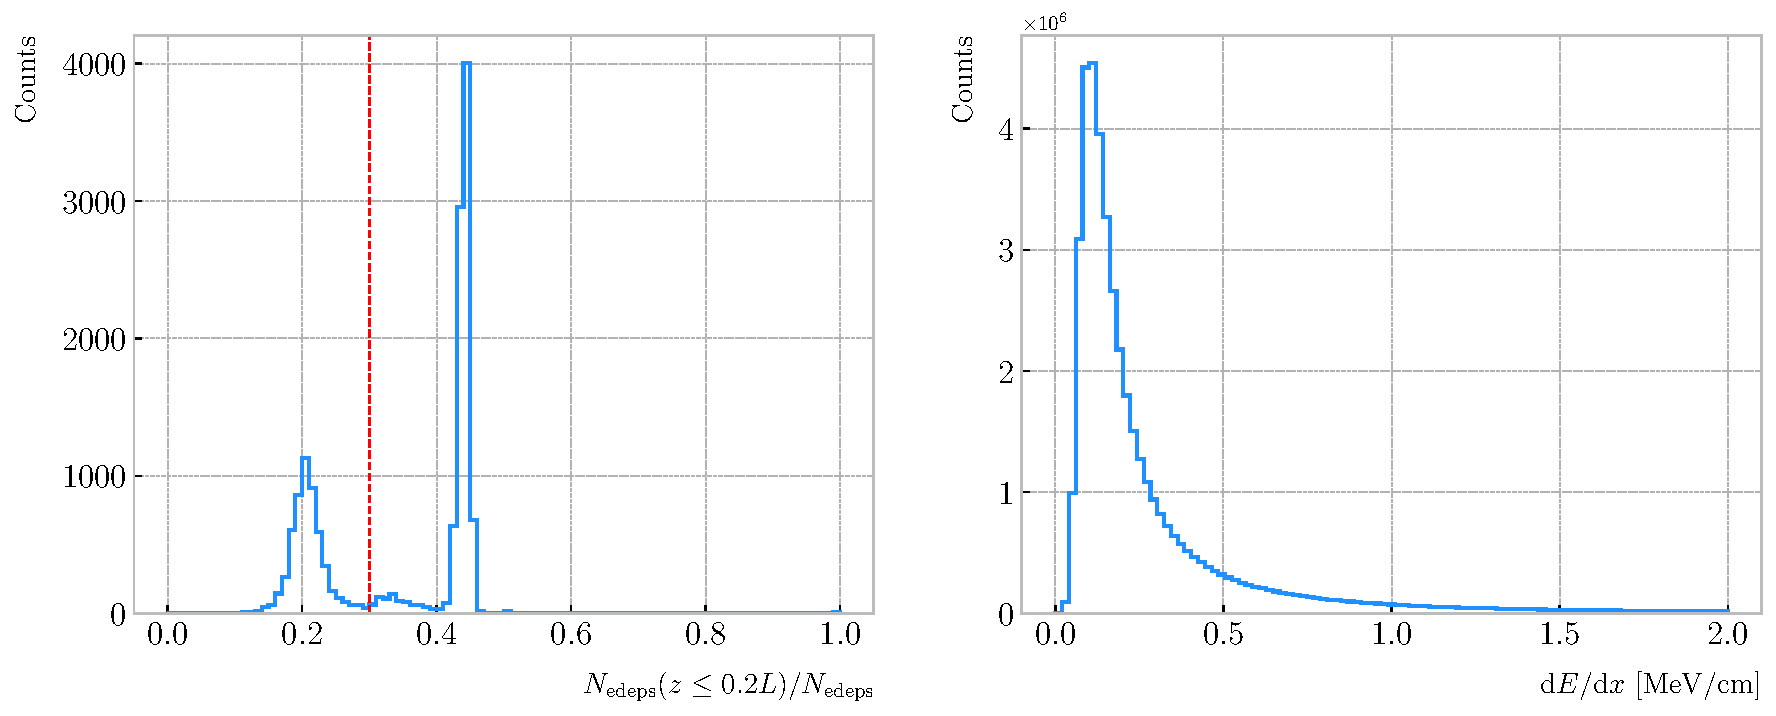
\includegraphics[width=.99\linewidth]{Images/GArSoft_Reco/dEdx/geant_selection_dEdx.pdf}
	\caption{Left panel: distribution of the fraction of Geant4-level energy deposits per track with residual range less than $20\%$ of the total track length, for the isotropic proton sample. Right panel: distribution of the ionisation per unit length of the energy deposits in the proton sample after removing the tracks with less than $30\%$ of their energy deposits in the last $20\%$ of the track.}
	\label{fig:geant_edeps}
\end{figure}

For studying the energy loss of the protons I select the reconstructed tracks that range out (i.e. slow down to rest) inside the TPC. A characteristic feature of the energy loss profile of any stopping ionising particle is the so-called Bragg peak, a pronounced peak that occurs immediately before the particle comes to rest. From Eq. (\ref{Eq:3.1}) we can see that this behaviour is expected, as the energy loss for non-relativistic particles is inversely proportional to $\beta^{2}$. In data, a way of identifying the Bragg peak, and thus select the stopping particles, is checking the number of energy deposits towards the end of the track. In this case, I count the fraction of the Geant4 simulated energy deposits with a residual range value (the distance from a given energy deposit to the last deposit in the track trajectory) less than a $20\%$ of the corresponding track length\footnote{As we are applying this selection at the Geant4 level we could have simply selected the stopping protons using the \texttt{EndProcess} labels from the simulation. However, the Bragg peak identification method displayed here could serve as a starting point for a selection of stopping protons in real data.}. The distribution of this fraction of energy deposits for our proton sample is shown in Fig. \ref{fig:geant_edeps} (left panel). We can clearly see two well separated peaks in this distribution, one centered at $0.2$ and another, narrower, one centered at a higher value. The first one corresponds to non-stopping protons, as in that case the number of energy deposits towards the end of the track is uniformly distributed due to the absence of the Bragg peak. In that way, I apply a cut in this distribution, requiring that at least $30\%$ of the simulated energy deposits sit in the last $20\%$ of the tracks, to ensure that the Bragg peak is present.

\begin{figure}[t]
	\begin{subfigure}{0.5\textwidth}
		\centering
		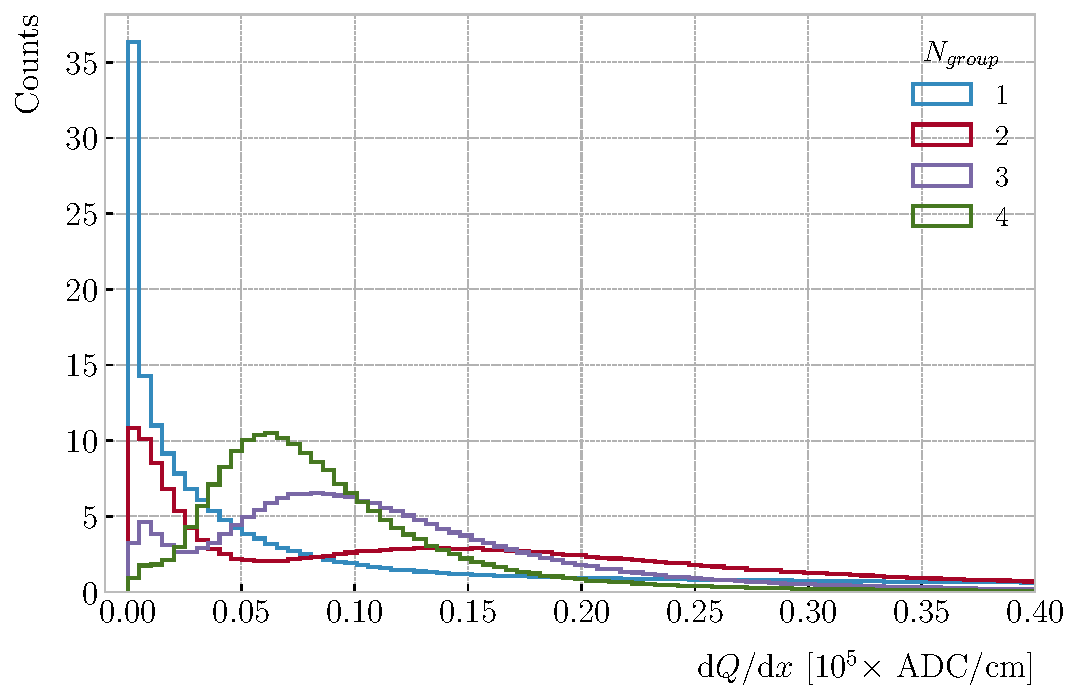
\includegraphics[width=.90\linewidth]{Images/GArSoft_Reco/dEdx/reco_dQdx_groups.pdf}
	\end{subfigure}
	\begin{subfigure}{0.5\textwidth}
		\centering
		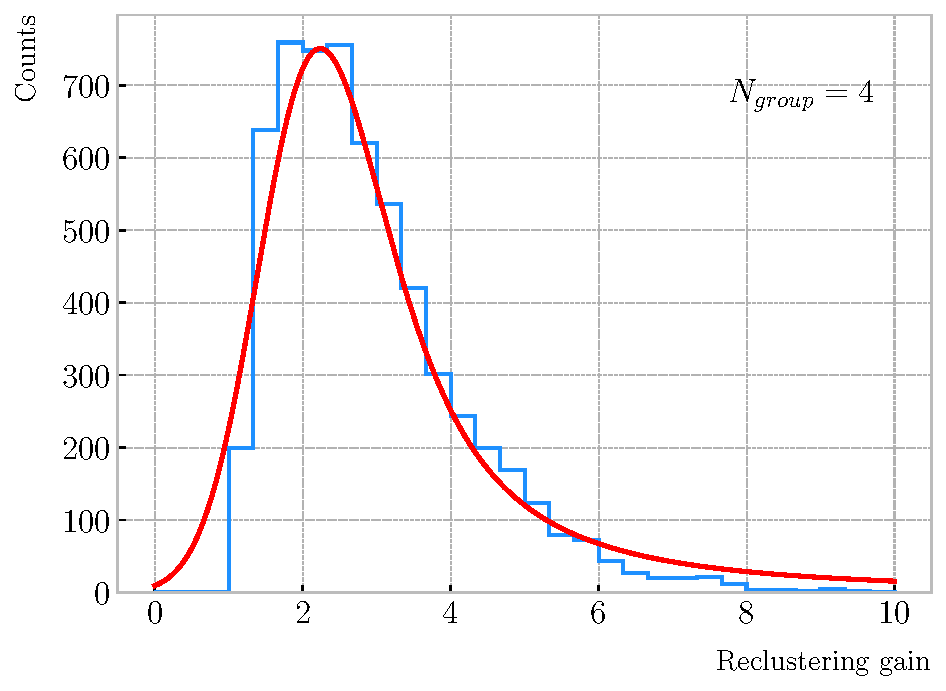
\includegraphics[width=.90\linewidth]{Images/GArSoft_Reco/dEdx/dQdx_recluster_gain.pdf}
	\end{subfigure}
	\caption{Left panel: distribution of the reconstructed ionisation charge per unit length for our MC stopping proton sample. The different colors indicate how many consecutive $\mathrm{d}Q/\mathrm{d}x$ pairs were grouped together. Right panel: distribution of the median change in $\mathrm{d}Q/\mathrm{d}x$ per track after $N_{group}=4$ clusters were reclustered together.}
	\label{fig:reco_dQ_groups}
\end{figure}

Fig. \ref{fig:geant_edeps} (right panel) shows the distribution of the energy loss per unit length for the Geant4 simulated energy deposits of the selected stopping protons. We can see that it follows the expected shape of a Landau distribution, which describes the fluctuations of the ionisation energy losses \cite{Landau1944}. This distribution has a characteristic asymmetric PDF, with a long right tail that translates into a high probability for high-energy ionisation losses. The origin of these fluctuations is mainly the possibility of transferring a high enough energy to an electron, so it becomes a ionising particle itself.

Now, from the point of view of the reconstruction, the objects that we have available to extract the ionisation information for the different reconstructed tracks are the collections of $\mathrm{d}Q$ and $\mathrm{d}x$ pairs, as stated before. The $\mathrm{d}Q$ values come from adding up the amplitude of all the reconstructed hits in a cluster, which is the input object to the Kalman fit.

Fig. \ref{fig:reco_dQ_groups} (left panel) shows the distribution of the ionisation charge deposits per unit length for the track in the stopping proton sample (blue line). As one can notice, this distribution does not resemble the expected shape of the Landau PDF. This distribution peaks sharply at $0$ and has a heavy tailed behaviour. Notice, however, how the distribution changes its shape as we group together $N_{group}$ consecutive charge deposit pairs (red, purple and green lines). The distribution in the $N_{group} = 4$ case already has a shape which resembles that of the Geant4-level ionisation per unit length, so I will proceed using this amount of reclustering for the reconstruction-level depositions.

An extra factor I need to account for, when reclustering is applied, is how the overall $\mathrm{d}Q/\mathrm{d}x$ per track changes. To do so, we can look at the ratio between the median $\mathrm{d}Q/\mathrm{d}x$ after and before the reclustering. Fig. \ref{fig:reco_dQ_groups} (right panel) shows the median enhancement in $\mathrm{d}Q/\mathrm{d}x$ per track for the stopping proton sample in the case $N_{group}=4$. From a Landau fit to this distribution, I estimate the most probable value of this ratio to be $G_{group} = 2.24$.

At this point, I am left with determining the conversion between the charge deposits per unit length $\mathrm{d}Q/\mathrm{d}x$ and the energy deposits per unit length $\mathrm{d}E/\mathrm{d}x$. To this end, we need a way of comparing the two. I can use the residual range $z$ to get a prediction of the most probable $\mathrm{d}E/\mathrm{d}x$ by using the following empirical parametrisation \cite{Ulmer2010}:
\begin{equation}\label{Eq:3.4}
	\frac{\mathrm{d}E}{\mathrm{d}x}(z) = \frac{z^{\frac{1}{p}-1}}{p\Lambda^{\frac{1}{p}}},
\end{equation}
which is quoted in the literature as the Bragg-Kleeman formula. In order to obtain the $p$ and $\Lambda$ parameters I perform a fit using the energy losses and the residual ranges given by the Geant4 stage of our proton sample.

Within our simulation, the residual range is sampled with a maximum size of $5~\mathrm{mm}$. Therefore, to perform the fit to the Bragg-Kleeman formula, we can use a fine-grained residual range binning. For each of the residual range bins I extract the $\mathrm{d}E/\mathrm{d}x$ distribution and fit it to a Landau distribution convolved with a Gaussian, to obtain the value of the most probable $\mathrm{d}E/\mathrm{d}x$ in the bin together with a statistical uncertainty. I then fit Eq. (\ref{Eq:3.4}) to these most probable values and the centres of the residual range bins. This procedure is depicted in Fig. \ref{fig:bragg_kleeman}, where I show the distribution of the energy loss per unit length versus the residual range, together with the most probable $\mathrm{d}E/\mathrm{d}x$ values and their uncertainty in each bin (golden points) and the curve with the best fit of the Bragg-Kleeman relation to those values (black line).

\begin{figure}[t]
	\centering
	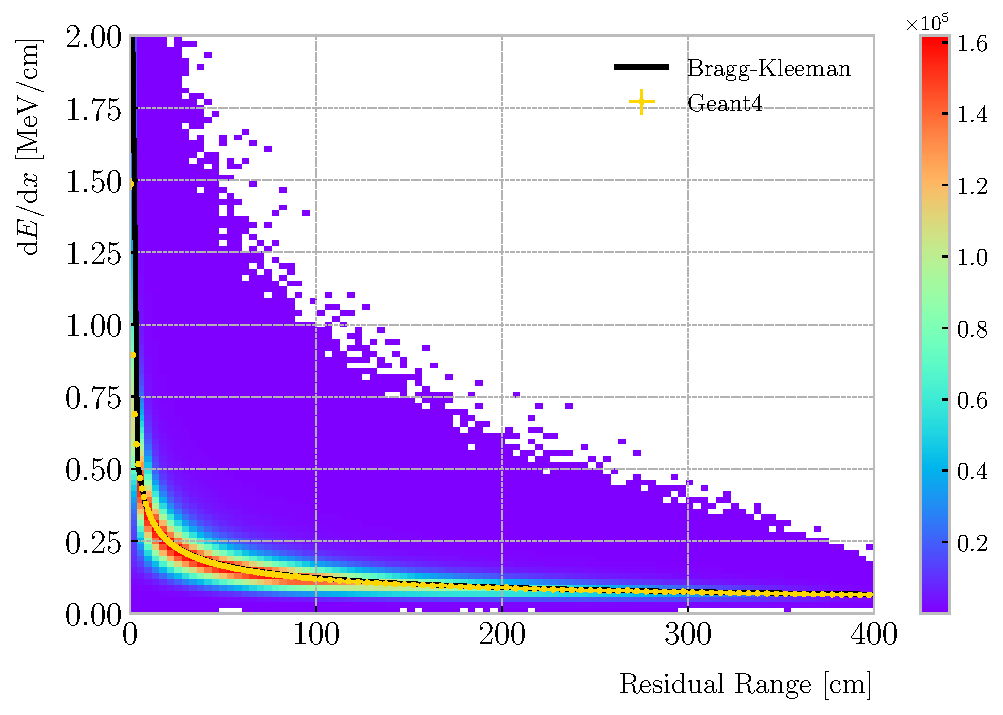
\includegraphics[width=.85\linewidth]{Images/GArSoft_Reco/dEdx/bragg_kleeman_geant_langau.pdf}
	\caption{Distribution of the Geant4-simulated energy losses per unit length versus residual range for the stopping proton sample. The overlaid points represent the fitted most probable value of the $\mathrm{d}E/\mathrm{d}x$ distribution in each residual range bin, whereas the curve is their best fit to the Bragg-Kleeman formula from Eq. (\ref{Eq:3.4}).}
	\label{fig:bragg_kleeman}
\end{figure}

Having an analytical expression that relates the residual range to $\mathrm{d}E/\mathrm{d}x$, I can take our reconstruction-level residual ranges from the stopping proton sample and compute the most probable energy loss associated.

In order to parametrise the charge saturation, we can use the following logarithmic function inspired by the modified box model for recombination:
\begin{equation}\label{Eq:3.5}
	\frac{\mathrm{d}E}{\mathrm{d}x} = \frac{\mathrm{e}^{\frac{\mathrm{d}Q}{\mathrm{d}x}B\frac{W_{ion}}{G_{group}C}}-A}{B},
\end{equation}
where $A$ and $B$ are the saturation parameters we need to determine, $W_{ion}$ is the average energy to produce an electron-ion pair, $G_{group}$ is the gain from the reclustering discussed above and $C$ is the calibration constant to convert number of electrons to ADC counts, commonly refer to as gain (also to be obtained in the fit). In this case, I use a value for the electron-ion production energy of $W_{ion} = 26.4 \ \mathrm{eV}$ \cite{Aprile2008}. This value, used in our simulation as well, was measured for gaseous argon in normal conditions, and therefore should be checked in the future to describe correctly the high-pressure argon-$\mathrm{CH}_{4}$ mixture of ND-GAr.

For the saturation fit I follow a procedure similar to the previous one for Eq. (\ref{Eq:3.4}). Binning the $\mathrm{d}E/\mathrm{d}x$ range, I fit a Landau distribution convolved with a Gaussian to the corresponding $\mathrm{d}Q/\mathrm{d}x$ distribution to obtain the most probable value. The resulting data points are shown in Fig. \ref{fig:energy_calibration} (red bars), the horizontal error bars depict the width of the $\mathrm{d}E/\mathrm{d}x$ bin whereas the vertical bars represent the error associated to the most probable value estimation. The fit to the logarithmic function in Eq. (\ref{Eq:3.5}) is also shown (black line), with a reduced chi-square value of $\chi^{2}/ndf=18.13$.

We can compare the value obtained for the gain with the one I use as input in the simulation. In GArSoft this value is set to $5 \ \mathrm{ADC}/e$ by default. The value of $4.94 \pm 0.49 \ \mathrm{ADC}/e$ that I get from the fit is in reasonable agreement with our expectation.

\begin{figure}[t]
	\centering
	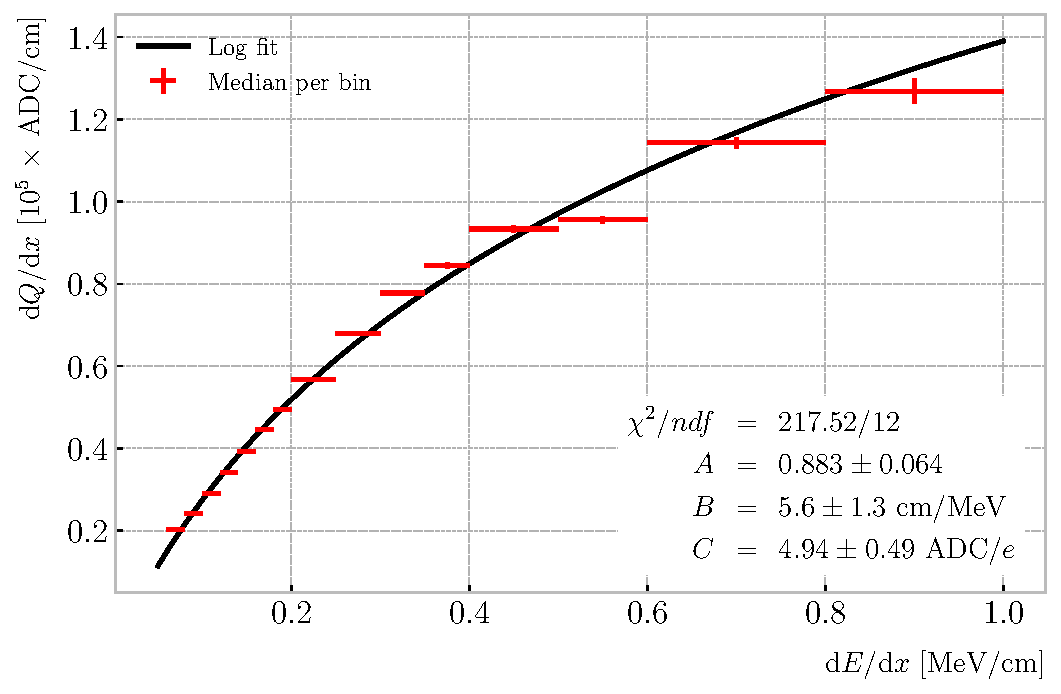
\includegraphics[width=.85\linewidth]{Images/GArSoft_Reco/dEdx/dEdx_vs_dQdx_log_fit.pdf}
	\caption{Distribution of the reconstructed ionisation charge per unit length for our MC stopping proton sample. The different colors indicate how many consecutive $\mathrm{d}Q/\mathrm{d}x$ pairs were grouped together.}
	\label{fig:energy_calibration}
\end{figure}

\begin{comment}
\begin{table}[h!]
	\caption{Effective recombination parameters obtained from the fit of ND-GAr simulated stopping proton sample to the modified box model. The corresponding parameters obtained by the LAr TPC experiments ArgoNeuT, $\mu$BooNE and ProtoDUNE are also shown for comparison.}
	\begin{center}
		\begin{tabular}{lcccc}
			\hline
																						   & ArgoNeuT        & $\mu$BooNE     & ProtoDUNE  & ND-GAr \\ \hline
			modified box model $\alpha$                                                    & $0.93\pm0.02$   & $0.92\pm0.02$  & $0.93\pm0.02$ & $0.91\pm0.02$       \\ \hline
			modified box model $\beta'$\\ $(\mathrm{kV/cm})(\mathrm{g/cm^{2}})/\mathrm{MeV}$ & $0.212\pm0.002$ & $0.184\pm0.02$ & $0.20\pm0.03$ & $0.040\pm0.004$     \\ \hline
			\end{tabular}
	\end{center}
	\label{tab:modified_box_fits}
\end{table}
\end{comment}

\section{Pion decay finding}

As discussed previously, in GArSoft the TPC tracks are formed after a pattern recognition algorithm and a Kalman filter are applied to the TPC clusters. These two steps can find discontinuities in the track candidates (e.g. due to a particle decay) when these so-called breakpoints are large enough. However, for some, more subtle, cases they may miss them and form a single reconstructed track. It has been noted in the literature that Kalman filters offer, as a by-product, additional information to form test statistics to identify these breakpoints \cite{Fruehwirth1988,Astier2000}.

\begin{figure}[t]
	\begin{subfigure}{0.5\textwidth}
		\centering
		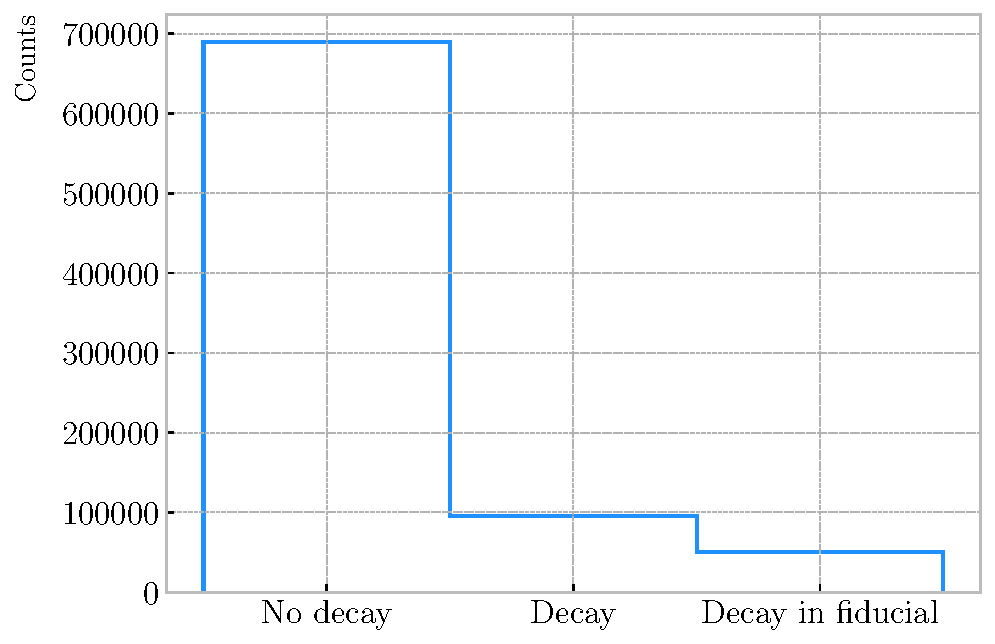
\includegraphics[width=.99\linewidth]{Images/GArSoft_Reco/pion_decay/pion_decay_status.pdf}
	\end{subfigure}
	\begin{subfigure}{0.5\textwidth}
		\centering
		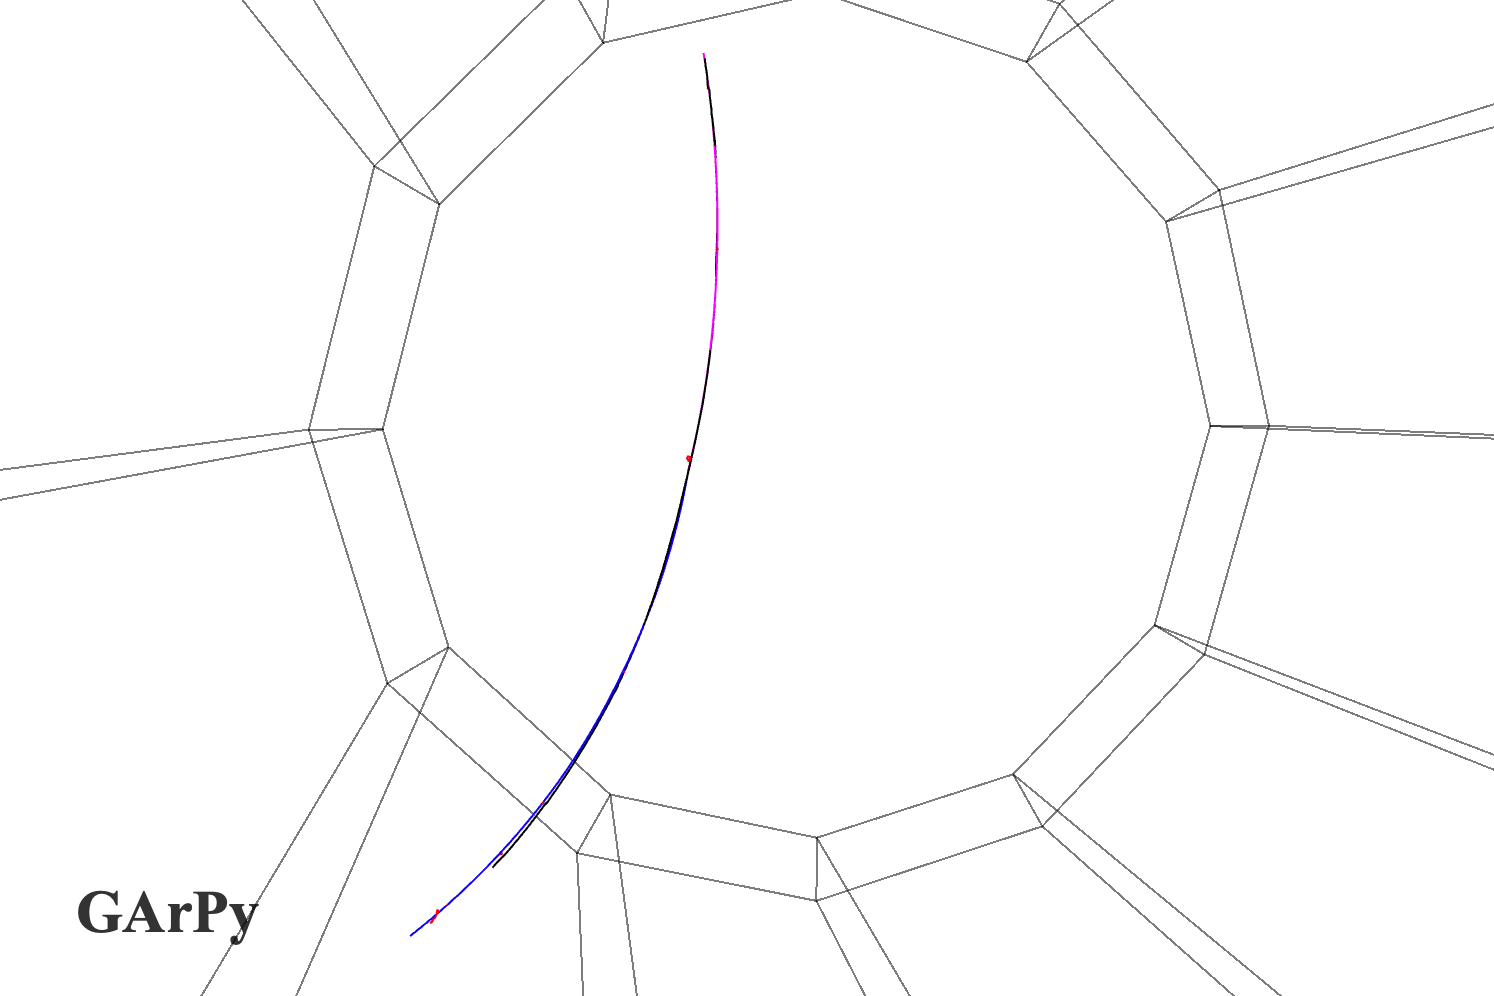
\includegraphics[width=.99\linewidth]{Images/GArSoft_Reco/pion_decay/pion_decay_evd.png}
	\end{subfigure}
	\caption{Left panel: number of non-decaying, decaying and decaying in the fiducial volume pions for a MC sample of $10^{5}$, $p=500 \ \mathrm{MeV}$ isotropic positively charged pions inside the TPC. Right panel: event display for a positive pion decaying inside the fiducial volume, with a single reconstructed track for the pion and muon system.}
	\label{fig:pion_decays}
\end{figure}

Considering the mean life of the charged pion, $\tau = (2.6033\pm0.0005)\times10^{-8} \ \mathrm{s}$, one can estimate that about $12\%$ of the pions with momentum $p \sim \mathcal{O}(500 \ \mathrm{MeV})$ (roughly the peak of the pion momentum distribution in $\nu_{\mu}$ CC interactions off argon) decay inside the TPC. Fig. \ref{fig:pion_decays} (left panel) shows the amount of charged pions decaying in the full TPC and fiducial volumes from an isotropic, monoenergetic sample of $10^{5}$ negatively charged pions with $p=500 \ \mathrm{MeV}$. We see that about $10\%$ of those decayed, with more than half of them decaying inside the TPC fiducial volume.

Fig. \ref{fig:pion_decays} (right panel) shows an example event display of a charged pion (magenta line) decays in flight inside the TPC, but because the angle of the muon (blue line) is small both were reconstructed as one single track (black line). In this case, the composite track reaches the ECal, where it undergoes a muon-like interaction, thus being classified as a muon.

A way to understand what decaying pion tracks were totally or partially reconstructed together with the daughter muon is looking at the relative energy contributions to the reconstructed track. In order to select a sample of such events, I require that a minimum $50\%$ of the total energy comes from the pion and at least $20\%$ from the muon.

To identify potential decays we can use the information we obtain from the Kalman filter at each step of the fitted track. The simplest test we can think about is computing the $\chi^{2}$ of the mismatch between all the parameters in the forward and the backward fits:
\begin{equation}
	\chi^{2 \ (FB)}_{k} = (\hat{\mathrm{x}}^{B}_{k}-\hat{\mathrm{x}}^{F}_{k})^{T}[V^{(\hat{\mathrm{x}}_{k},B)}+V^{(\hat{\mathrm{x}}_{k},F)}]^{-1}(\hat{\mathrm{x}}^{B}_{k}-\hat{\mathrm{x}}^{F}_{k}),
\end{equation}
where $\hat{\mathrm{x}}^{F}_{k}$, $\hat{\mathrm{x}}^{B}_{k}$ are the Kalman filter state vector estimates at step $k$ in the forward and backward fits and $V^{(\hat{\mathrm{x}}_{k},F)}$, $V^{(\hat{\mathrm{x}}_{k},B)}$ the covariance matrices of $\hat{\mathrm{x}}^{F}_{k}$ and $\hat{\mathrm{x}}^{B}_{k}$ respectively. Using the values of the $\chi^{2}$ at measurement $k$ for the forward and backward fits we can compute another $\chi^{2}$ value that characterises the overall track fit:
\begin{equation}
	\chi^{2}_{track} = \chi^{2 \ (F)}_{k} + \chi^{2 \ (B)}_{k} + \chi^{2 \ (FB)}_{k},
\end{equation}
which remains approximately constant for all $k$.

An alternative approach proposed in the context of the NOMAD experiment was using a fit with a more elaborate breakpoint hypothesis, so we can perform a comparison of the $\chi^{2}$ with and without breakpoints. This can be achieved by using some alternative parametrisation with extra parameters, which allows some of the track parameters to be discontinuous at certain points. A decay changes the momentum magnitude and direction, so we can use the new state vector:
\begin{equation}
	\alpha=\begin{pmatrix}y,& z,& 1/R_{F},& 1/R_{B},& \phi_{F},& \phi_{B},& \mathrm{tan}\lambda_{F},& \mathrm{tan}\lambda_{B}\end{pmatrix}^{T}.
\end{equation}

\begin{figure}[t]
	\centering
	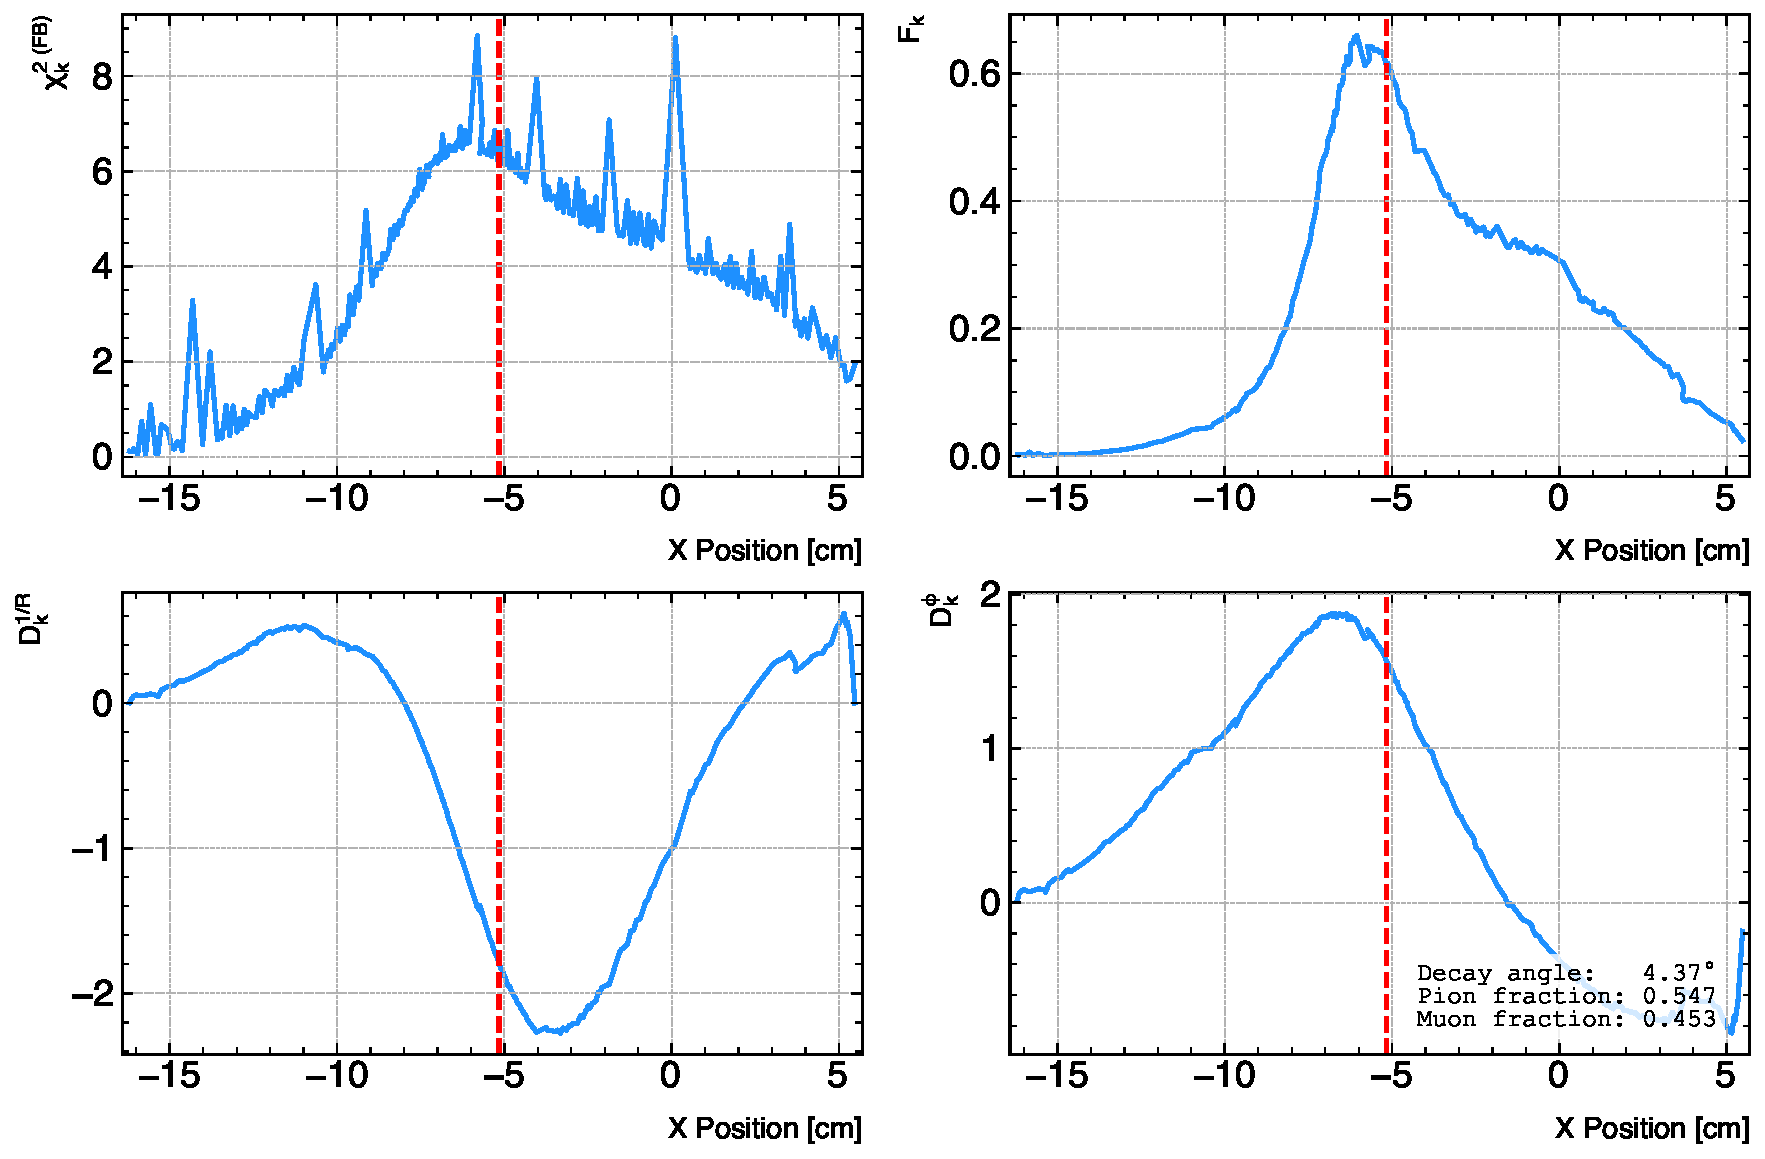
\includegraphics[width=.85\linewidth]{Images/GArSoft_Reco/pion_decay/pion_decay_variables_event_425.pdf}
	\caption{Values of $\chi^{2 \ (FB)}_{k}$ (top left panel), $F_{k}$ (top right panel), $D^{1/R}_{k}$ (bottom left panel) and $D^{\phi}_{k}$ (bottom right panel) versus position along the drift direction for a reconstructed track in a positive pion decay event. The vertical red dashed line indicates the true location of the decay point.}
	\label{fig:breakpoint_variables_example}
\end{figure}

As we already have the estimates from the standard Kalman filter and their covariance matrices at each point, we do not need to repeat the Kalman fit for the new parametrisation. Instead, I can compute the values of $\alpha$ at each point $k$ that minimise the $\chi^{2}$ resulting from comparing them to $\{\hat{\mathrm{x}}^{B}_{k}, \hat{\mathrm{x}}^{F}_{k}\}$. Introducing the two $5 \times 8$ matrices:
\begin{equation}
	H^{F}=\begin{pmatrix}1&0&0&0&0&0&0&0 \\ 0&1&0&0&0&0&0&0 \\ 0&0&1&0&0&0&0&0 \\ 0&0&0&0&1&0&0&0 \\ 0&0&0&0&0&0&1&0\end{pmatrix}, \
	H^{B}=\begin{pmatrix}1&0&0&0&0&0&0&0 \\ 0&1&0&0&0&0&0&0 \\ 0&0&0&1&0&0&0&0 \\ 0&0&0&0&0&1&0&0 \\ 0&0&0&0&0&0&0&1\end{pmatrix},
\end{equation}
we can write this as:
\begin{equation}
	\begin{split}
		\chi_{k}^{2 \ (FB)} (\alpha) &= (\hat{\mathrm{x}}_{k}^{F}-H^{F}\alpha)^{T}\left[V^{(\hat{\mathrm{x}}_{k},F)}\right]^{-1}(\hat{\mathrm{x}}_{k}^{F}-H^{F}\alpha)\\
		&+(\hat{\mathrm{x}}_{k}^{B}-H^{B}\alpha)^{T}\left[V^{(\hat{\mathrm{x}}_{k},B)}\right]^{-1}(\hat{\mathrm{x}}_{k}^{B}-H^{B}\alpha).
	\end{split}
\end{equation}

The minimum of $\chi_{k}^{2 \ (FB)} (\alpha)$ is found when the measured new state vector takes the value:
\begin{equation}
	\hat{\alpha}_{k} = V^{(\hat{\alpha}_{k})} H^{T} (V^{(\hat{\mathrm{x}}_{k})})^{-1} \hat{\mathrm{X}},
\end{equation}
where $\hat{\mathrm{X}} = \{\hat{\mathrm{x}}^{B}_{k}, \hat{\mathrm{x}}^{F}_{k}\}$, $V^{(\hat{\mathrm{x}}_{k})}$ is the block diagonal matrix formed by $V^{(\hat{\mathrm{x}}_{k},F)}$ and $V^{(\hat{\mathrm{x}}_{k},B)}$ and $V^{(\hat{\alpha}_{k})}$ is the covariance matrix of $\hat{\alpha}_{k}$, given by:
\begin{equation}
	V^{(\hat{\alpha}_{k})} = \left(H^{T} (V^{(\hat{\mathrm{x}}_{k})})^{-1} H\right)^{-1}.
\end{equation}

\begin{figure}[t]
	\begin{subfigure}{0.5\textwidth}
		\centering
		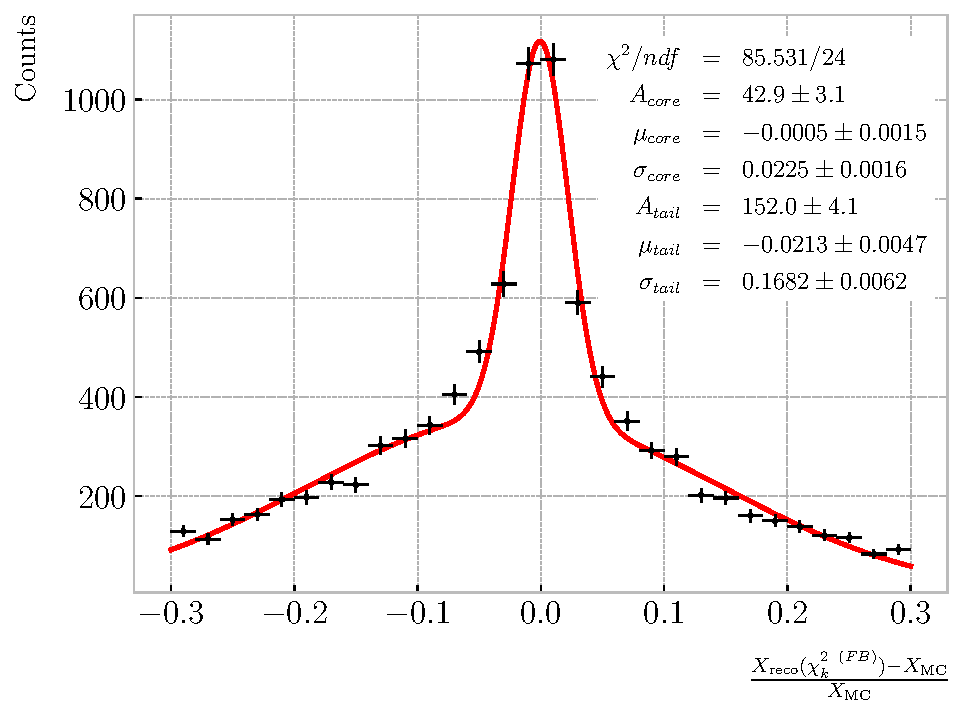
\includegraphics[width=.99\linewidth]{Images/GArSoft_Reco/pion_decay/pion_decay_resolution_chisqfb.pdf}
	\end{subfigure}
	\begin{subfigure}{0.5\textwidth}
		\centering
		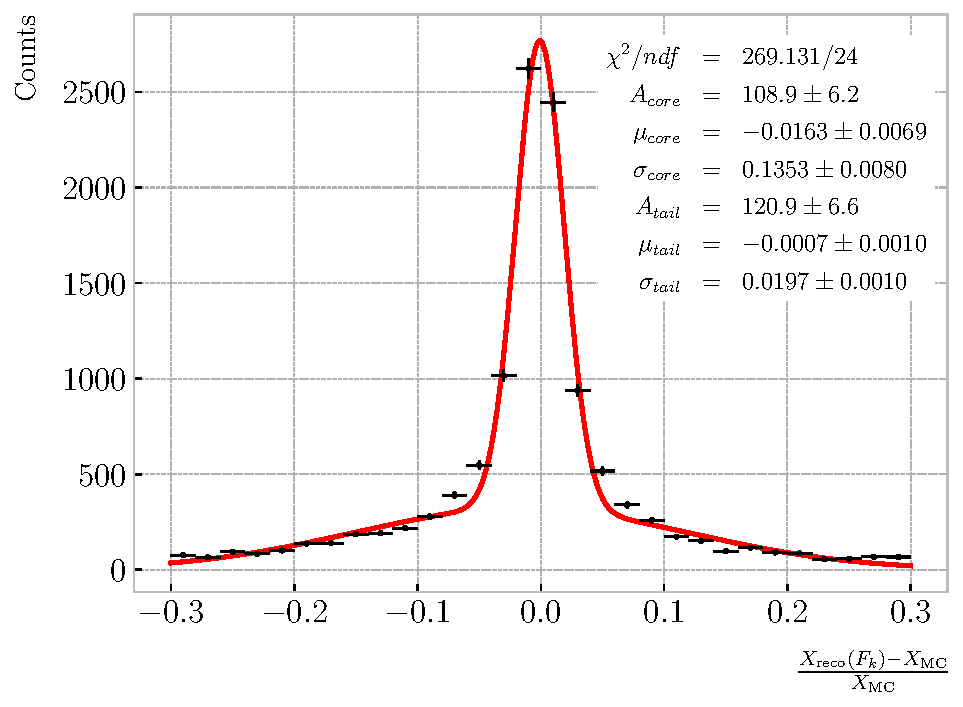
\includegraphics[width=.99\linewidth]{Images/GArSoft_Reco/pion_decay/pion_decay_resolution_fisher.pdf}
	\end{subfigure}
	\caption{Fractional residual distributions of the true and reconstructed decay position along the drift coordinate, using the position of the maximum of $\chi^{2 \ (FB)}_{k}$ (left panel) and $F_{k}$ (right panel) as estimates of the decay position. Also shown are double Gaussian fits to these points (red lines).}
	\label{fig:pion_decay_resolution}
\end{figure}

From these new fit estimates we can compute the $F$ statistic, which tells us whether the model with breakpoint provides a statistically significant better fit:
\begin{equation}
	F_{k}=\left(\frac{\chi^{2}_{track,k}-\chi^{2}_{full,k}}{8-5}\right)/\left(\frac{\chi^{2}_{full,k}}{N-8}\right).
\end{equation}

One can also compute the signed difference of the duplicated variables divided by their standard deviation at each point. These represent how significant the discontinuity in each variable is. For any variable $\eta$ we can write it as:
\begin{equation}
	D^{\eta}_{k} = \frac{\hat{\eta}^{B}_{k}-\hat{\eta}^{F}_{k}}{\sqrt{\mathrm{Var}[\hat{\eta}^{F}_{k}]+\mathrm{Var}[\hat{\eta}^{B}_{k}]-2\mathrm{Cov}[\hat{\eta}^{F}_{k}, \hat{\eta}^{B}_{k}]}}.
\end{equation}
In our case, the relevant ones to look at are $D^{1/R}_{k}$ and $D^{\phi}_{k}$.

Fig. \ref{fig:breakpoint_variables_example} shows the values of $\chi^{2 \ (FB)}_{k}$, $F_{k}$, $D^{1/R}_{k}$ and $D^{\phi}_{k}$ as functions of the position along the drift direction, for an example reconstructed track with $55.5\%$ of the energy coming from the charged pion and $45.5\%$ from the daughter muon. The true position of the decay is indicated (dashed red lines). Notice how $\chi^{2 \ (FB)}_{k}$ and $F_{k}$, $D^{1/R}_{k}$ reach their maxima near the decay point. In the former case this indicates a large forward-backward difference in the track fit. In the later it represents that the extended state vector improves the fit particularly around that point.

I can estimate the decay position finding resolution by computing the difference between the $X$ position of the maxima of $\chi^{2 \ (FB)}_{k}$ and $F_{k}$ and the $X$ position of the true decay. Fig. \ref{fig:pion_decay_resolution} represent the  the fractional residual distributions for both cases, from the sample of tracks containing pion decays. Fitting a double Gaussian to the distributions (red lines) I find a resolution of $13.62\%$ and $7.45\%$ respectively.

In principle, the $F$-statistic should follow a Fisher distribution with $(8-5)$ and $(N-8)$ degrees of freedom under the null hypothesis. In most of our cases $N\sim\mathcal{O}(100)$, so the probability density functions will look very similar. In this case, it is safe to take the limit $N\rightarrow\infty$ in the Fisher PDF:
\begin{equation}
	\begin{split}
		\tilde{f}(x;a-b)&=\lim_{N \rightarrow \infty} f(x;a-b,N-a)\\
		&= \frac{2^{-\frac{a-b}{2}}}{\Gamma\left(\frac{a-b}{2}\right)}\left(a-b\right)^{\frac{a-b}{2}}x^{\frac{a-b}{2}-1}\mathrm{e}^{-\frac{a-b}{2}x}.
	\end{split}
\end{equation}
In our case $a-b = 8-5 = 3$, so we would obtain a p-value of $0.05$ at $x=2.60$.

\begin{figure}[t]
	\centering
	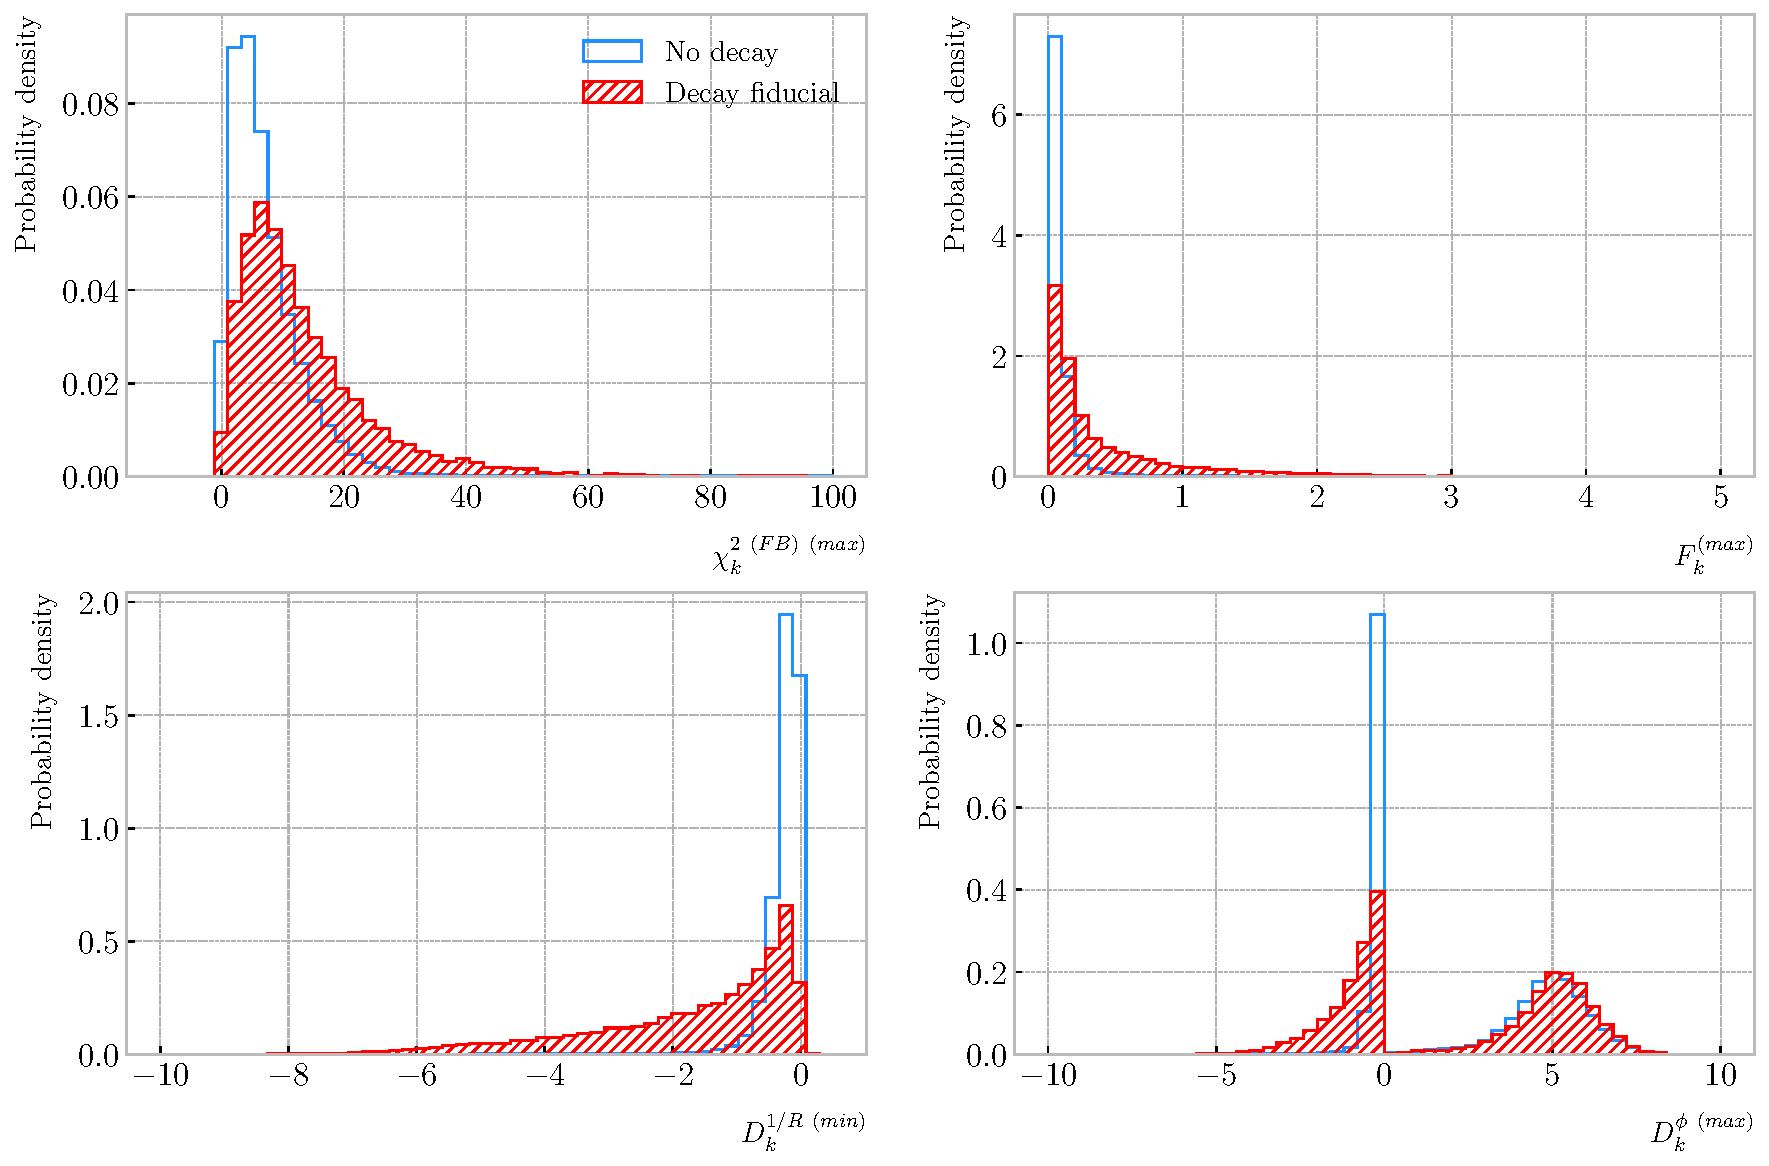
\includegraphics[width=.85\linewidth]{Images/GArSoft_Reco/pion_decay/pion_decay_variables.pdf}
	\caption{Distributions of the extreme values of $\chi^{2 \ (FB)}_{k}$ (top left panel), $F_{k}$ (top right panel), $D^{1/R}_{k}$ (bottom left panel) and $D^{\phi}_{k}$ (bottom right panel) for non-decaying reconstructed pion tracks (blue) and tracks which include the decay inside the fiducial volume (red).}
	\label{fig:breakpoint_variables}
\end{figure}

Fig. \ref{fig:breakpoint_variables} contains the distributions of the maxima of $\chi^{2 \ (FB)}_{k}$, $F_{k}$ and $D^{\phi}_{k}$ and the minima of $D^{1/R}_{k}$ for a sample of non-decaying pion tracks (blue) and another sample of reconstructed tracks containing part of the pion and the daughter muon from a decay inside the fiducial volume (red). Notice that, even though the values of $F^{(max)}_{k}$ for the decay sample are typically larger than for the non-decaying one, just a small fraction of the events go beyond the aforementioned value of $F=2.60$. Therefore, from a practical point of view, it is not the most efficient variable to use for selecting the decay events.

However, looking at the $D^{1/R \ (min)}_{k}$ distribution we can see there is a big difference between non-decaying and decaying events in this variable. One can use a combination of these four variables to distinguish between the pion decay events (signal) and the non-decaying pions (background).

\begin{figure}[t]
	\centering
	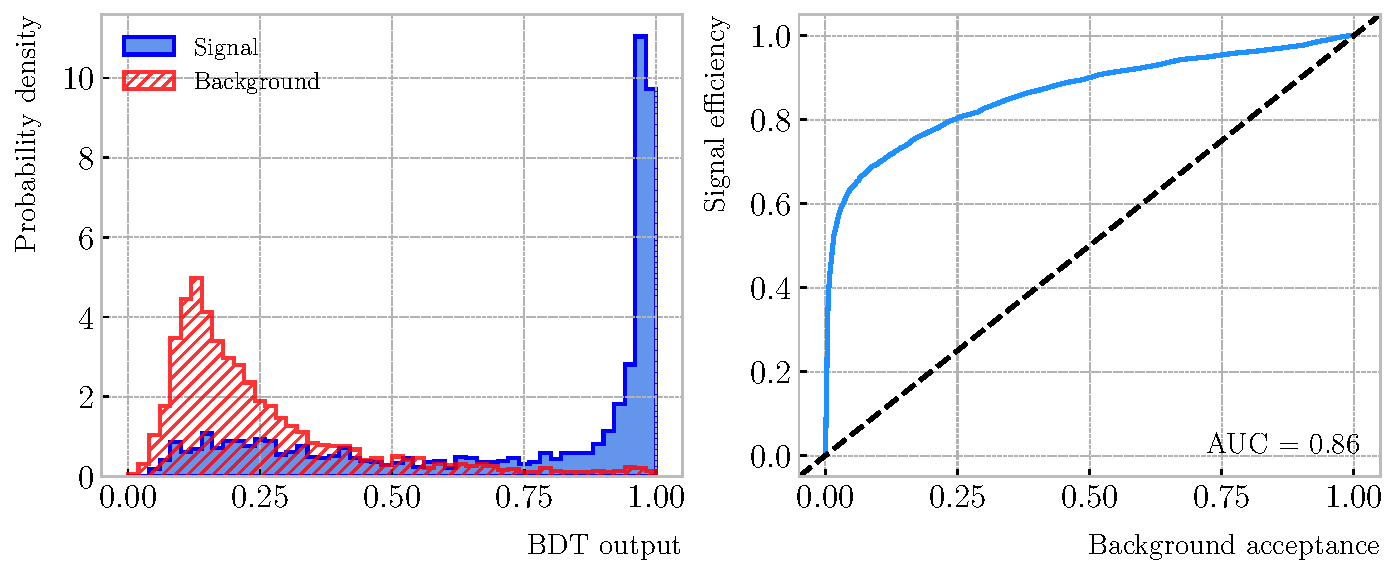
\includegraphics[width=.85\linewidth]{Images/GArSoft_Reco/pion_decay/pion_decay_summary_bdt.pdf}
	\caption{Left panel: distributions of the predicted probabilities assigned by the BDT classifier to a test sample of decaying pion+muon tracks (blue) and non-decaying pion tracks (red). Left: signal efficiency versus background acceptance (ROC curve) obtained from the BDT for the test sample.}
	\label{fig:breakpoint_bdt}
\end{figure}

\begin{figure}[t]
	\centering
	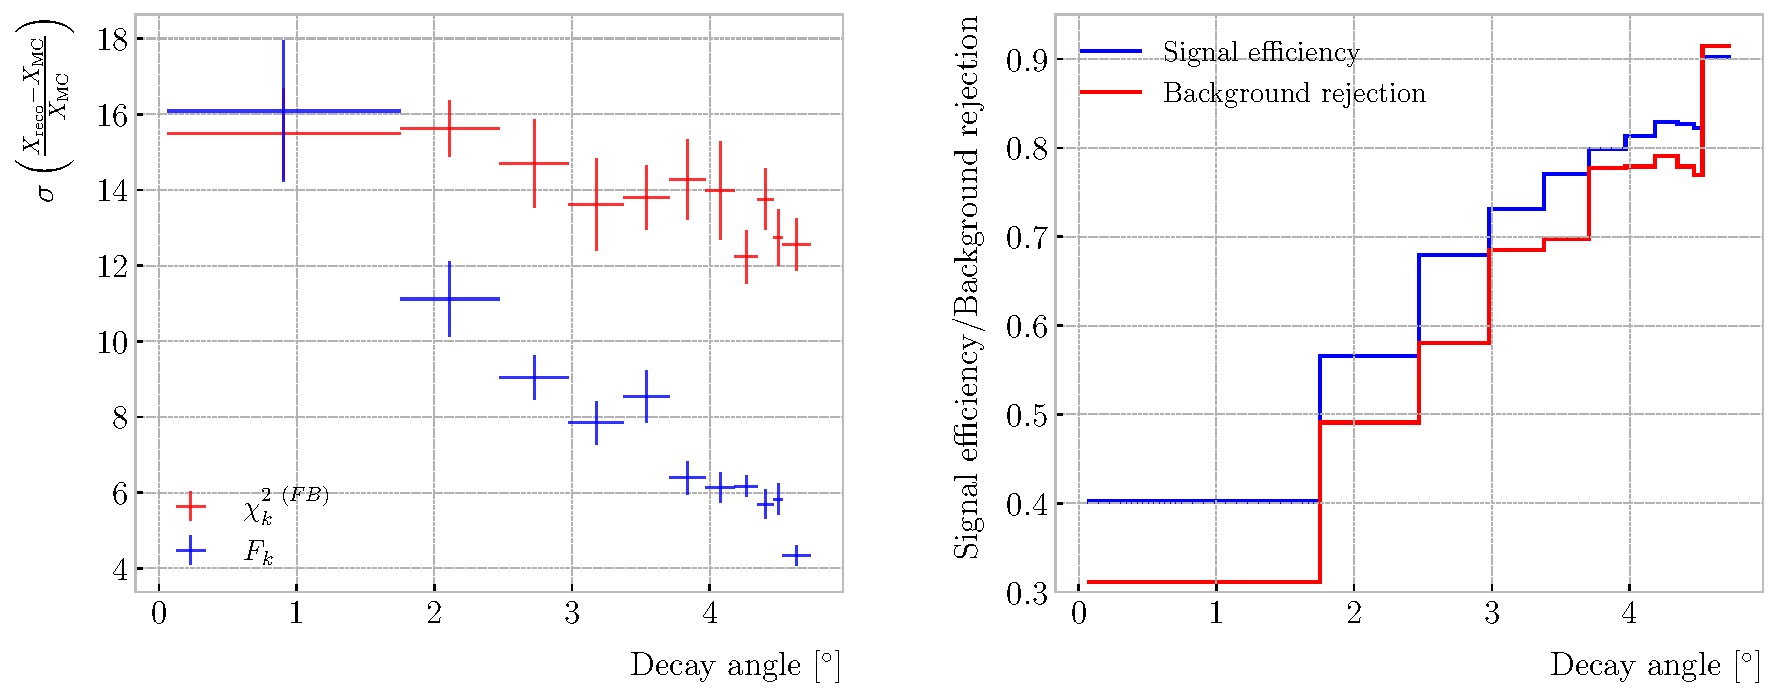
\includegraphics[width=.85\linewidth]{Images/GArSoft_Reco/pion_decay/pion_decay_angle_summary2.pdf}
	\caption{Left panel: dependence of the decay position finding resolution on the true value of the decay angle for the $\chi_{k}^{2 \ (FB)}$ (red) and $F_{k}$ (blue) methods. Right panel: signal efficiency (blue line) and background rejection (red line) from the BDT classifier versus true decay angle.}
	\label{fig:breakpoint_angle}
\end{figure}

An approach to this classification could be using a boosted decision tree (BDT). One of the advantages of BDTs is that they are easy to interpret and identify the relative importance of the different input variables. Training a BDT with $400$ estimators and a maximum depth of $4$ I can obtain an efficient classification without overtraining. Fig. \ref{fig:breakpoint_bdt} (left panel) shows the distribution of probabilities predicted by the BDT for a test sample. The signal efficiency as a function of background acceptance, the so-called ROC curve, is shown in Fig. \ref{fig:breakpoint_bdt} (right panel). With a relative importance of $0.83$, the most important variable turned out to be $D_{k}^{1/R \ (min)}$.

One thing we can check is how the resolution to the decay and the signal efficiency in the classification changes with the true decay angle. Using an equal-frequency binning for the decay angles, we can repeat the previous steps for each bin.

Fig. \ref{fig:breakpoint_angle} (left panel) shows the dependence on the decay angle of the decay finding resolution. We can see that for the $\chi_{k}^{2 \ (FB)}$ maximum location method the resolution consistently lies between $12$ to $16\%$. However, the $F^{(max)}_{k}$ approach gives a significantly better resolution for high angle values, reaching the $4-6\%$ range for decay angles $\geq 4^{\circ}$.

For the classification dependence on the angle, I use the same classifier I trained before but evaluating the test sample for each individual angular bin. I compute the signal efficiency in each bin for a fixed value of the background rejection, in this case $90\%$. Similarly, for the background rejection estimation I use a fixed signal efficiency value of $90\%$. Fig. \ref{fig:breakpoint_angle} (right panel) represents the change in signal efficiency (blue) and background rejection (red) with the value of the true decay angles.

\begin{figure}[t]
	\centering
	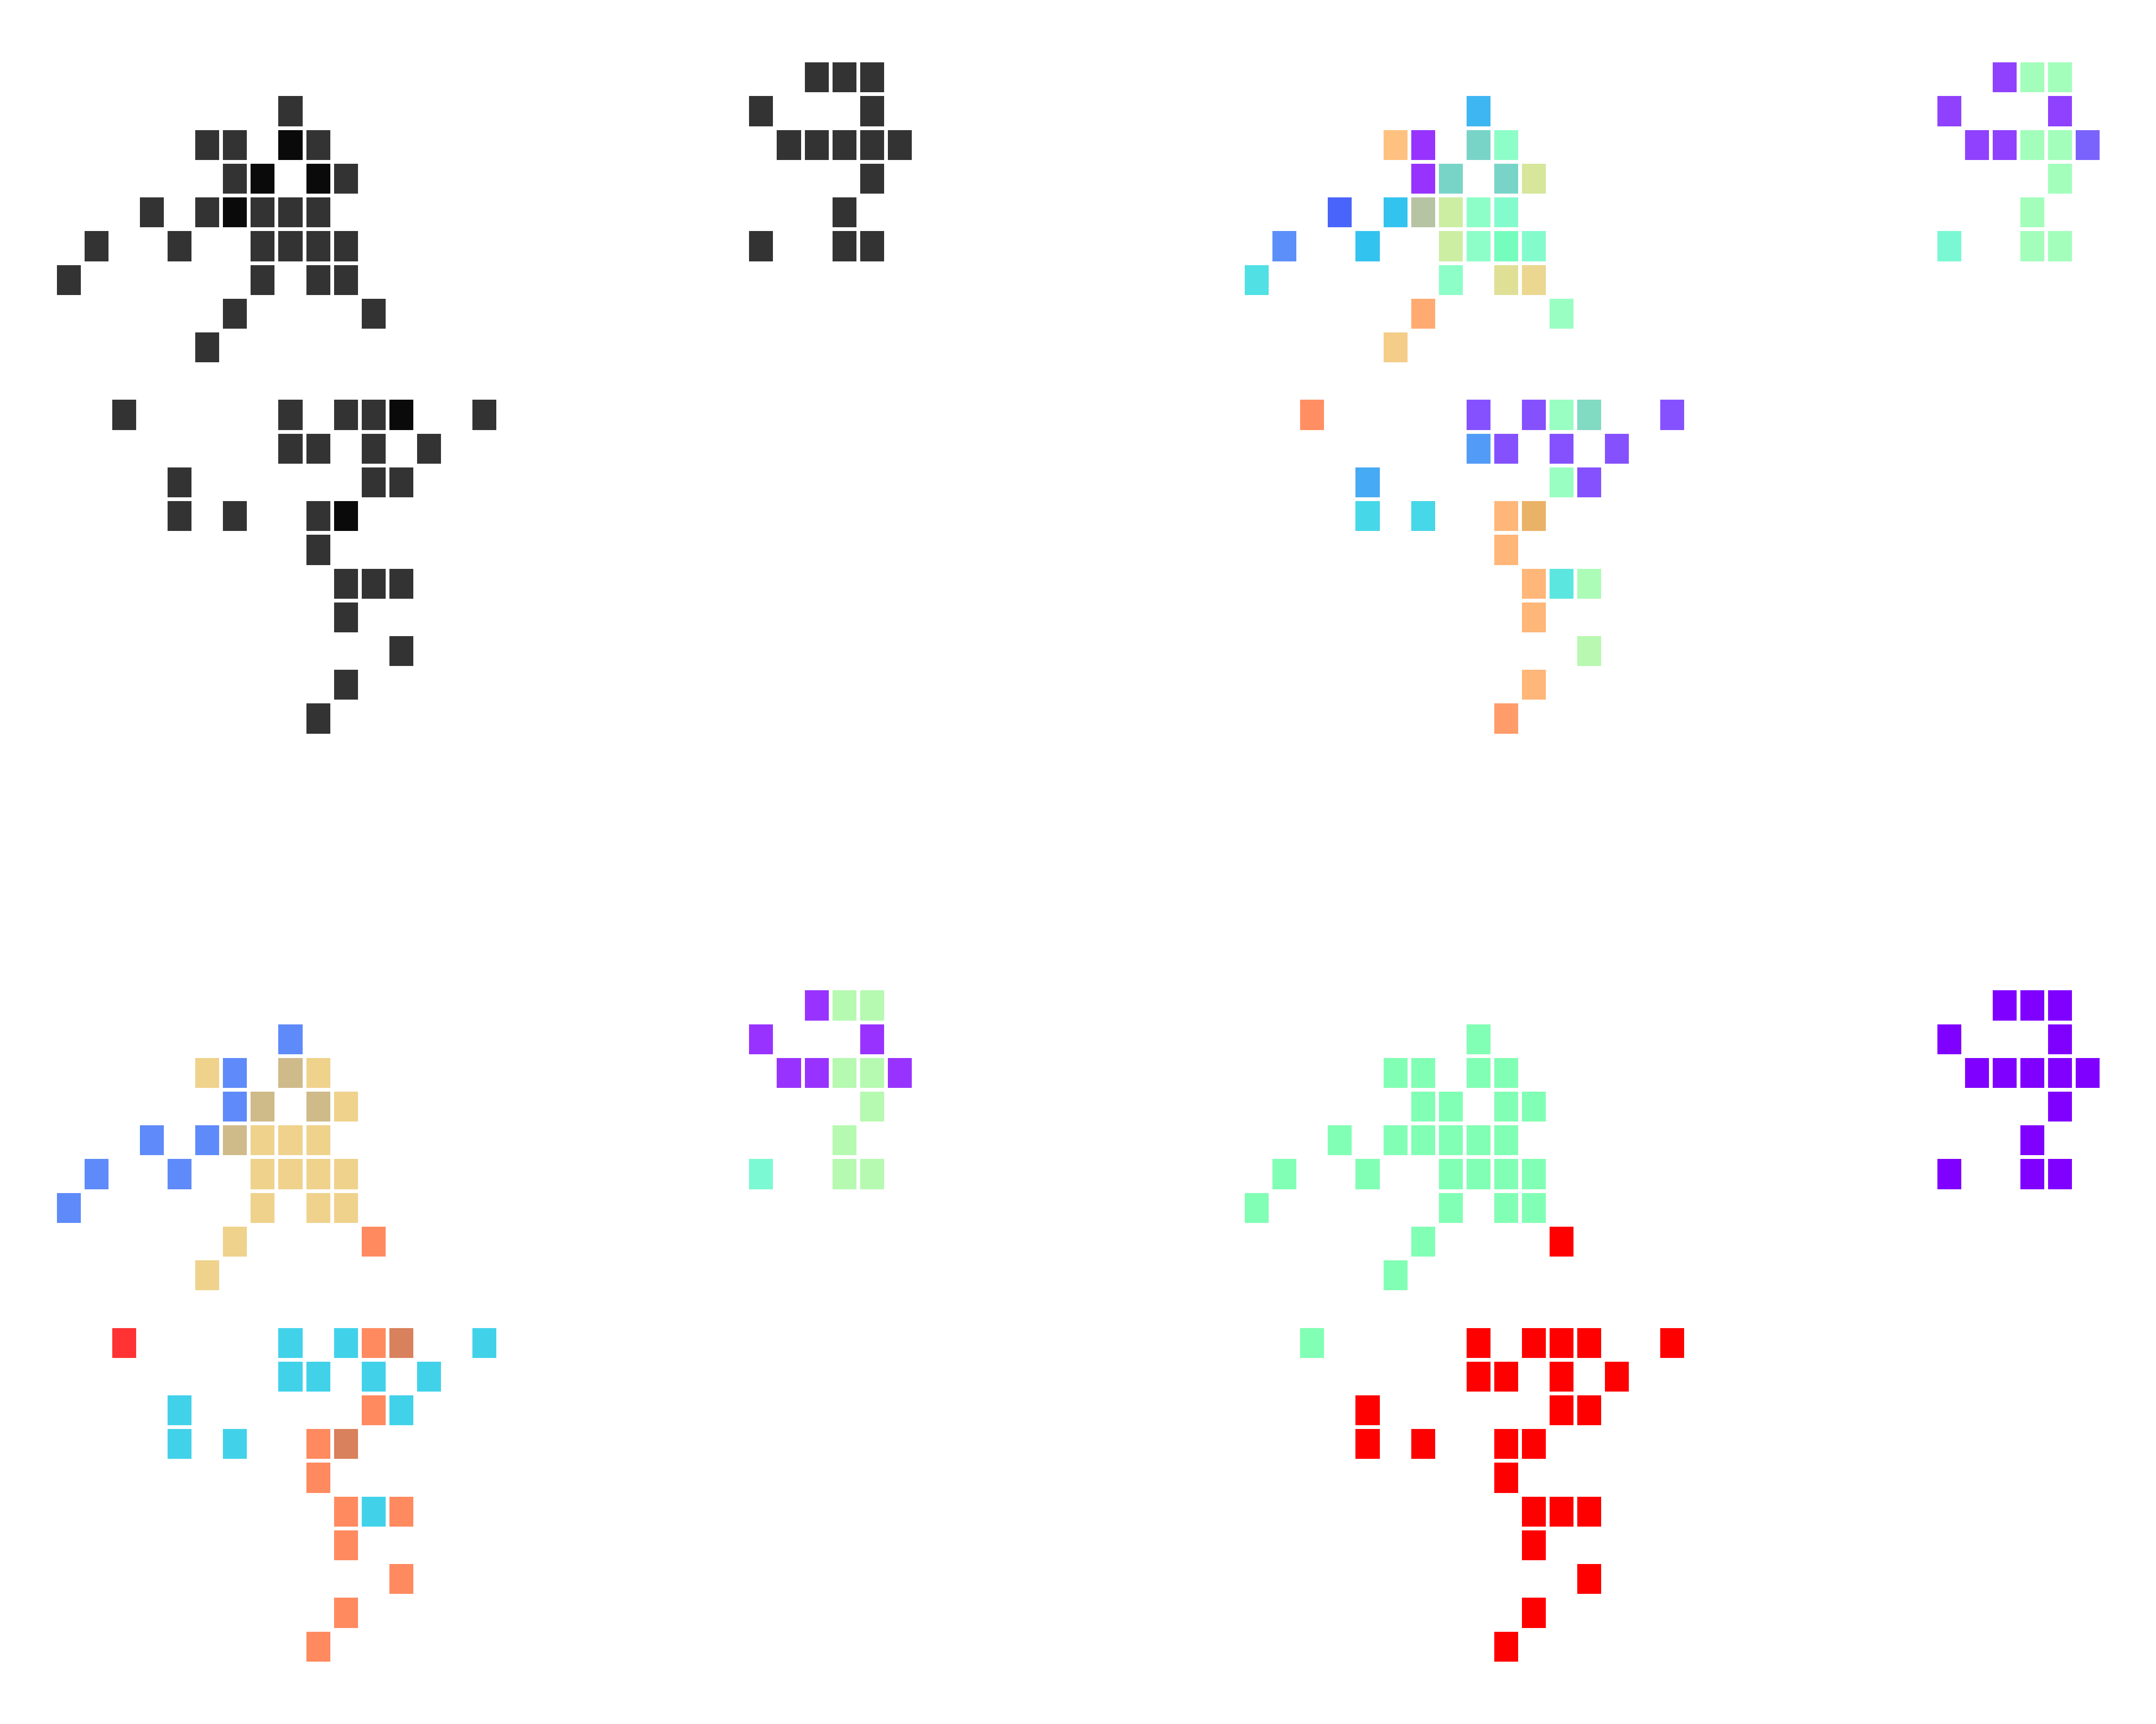
\includegraphics[width=.90\linewidth]{Images/GArSoft_Reco/cluster/cluster_primitive_recluster_example.png}
	\caption{Example clustering steps for the strip layers of an ECal barrel module in a $\nu_{\mu}$ CC interaction. From the top left to the right: input hits, NN clustering, re-clustering and strip view merging. The two clusters on the left correspond to a photon pair from a $\pi^{0}$ decay, whereas the one on the right comes from a proton.}
	\label{fig:clustering_example}
\end{figure}

\section{ECal clustering}

Another important reconstruction item is the clustering algorithm of ECal hits in GArSoft. The default module features a NN algorithm that treats all hits in the same way, independently of the layer each hit comes from. However, the current ECal design of ND-GAr has two very different types of scintillator layers. The inner layers are made out of tiles, which provide excellent angular and timing resolutions. On the other hand, the outer layers are cross scintillator strips. That way, an algorithm that treats hits from both kinds of layers differently may be able to improve the current performance.

Inspired by the reconstruction of T2K's ND280 downstream ECal \cite{T2KUK2013}, the idea was to put together a clustering module that first builds clusters for the different ECal views (tiles, strips segmented in the $X$ direction and strips segmented in $Y$ direction), and then tries to match them together to form the final clusters.

Working on a module-by-module basis, the algorithm first separates the hits depending on the layer type they come from. Then, it performs a NN clustering for the 3 sets of hits separately. For the tile hits it clusters together all the hits which are in nearest-neighbouring tiles and nearest-neighbouring layers, for strip hits it looks at nearest-neighbouring strips and next-to-nearest-neighbouring layers (as the layers with strips along the two directions are alternated). For strip clusters an additional cut in the direction along the strip length is needed.

After this first clustering I then apply a recursive re-clustering for each collection of strip clusters based on a PCA method. In each case, we loop over the clusters with $N_{hits}\geq2$, computing the centre of mass and three principal components. Propagating these axes up to the layers of the rest of the clusters, we check if the propagated point and the centre of mass of the second cluster are within next-to-nearest-neighbouring strips. An additional cut in the direction along the strip length is also needed. Moreover, I require that the two closest hits across the two clusters are at most in next-to-nearest-neighbouring strips. I merge the clusters if these three conditions are satisfied. The re-clustering is repeated until no more cluster pairs pass the cuts.

The clusters in each strip view are combined if their centres of mass are close enough and they point in the same direction. An alternative approach for the strip cluster merging could be to compute the overlap between the ellipsoids defined by the principal axes of the clusters, and then merge the pair if the overlap exceeds some threshold. Further study is needed to understand if this change would have an impact in the overall clustering performance.

To merge the tile clusters to the combined strip clusters I propagate the principal axis of the strip cluster towards the inner layers, up to the centre of mass layer of the tile cluster. I merge the clusters if the distance between the propagated point and the centre of mass is bellow a certain cut.

The last step is to check if clusters in neighbouring modules should be merged together, both across two barrel modules, across end cap modules and between barrel end cap modules. I check the distance between the two closest hits in the pair of clusters and merge them if it passes this and an additional direction cut.

Fig. \ref{fig:clustering_example} presents an example of the clustering steps relevant for strip layer hits, from the input hits (top left panel) to the NN clustering (top right panel) and re-clustering (bottom left panel) for each strip view and the final merging strip clusters (bottom right panel). It shows the hits from a single ECal barrel module in a $\nu_{\mu}$ CC interaction event with a neutral pion and a proton in the final state. The two clusters on the left correspond to the photon pair from the $\pi^{0}$ decay and the one on the upper right corner is associated to the proton.

\begin{figure}[t]
	\centering
	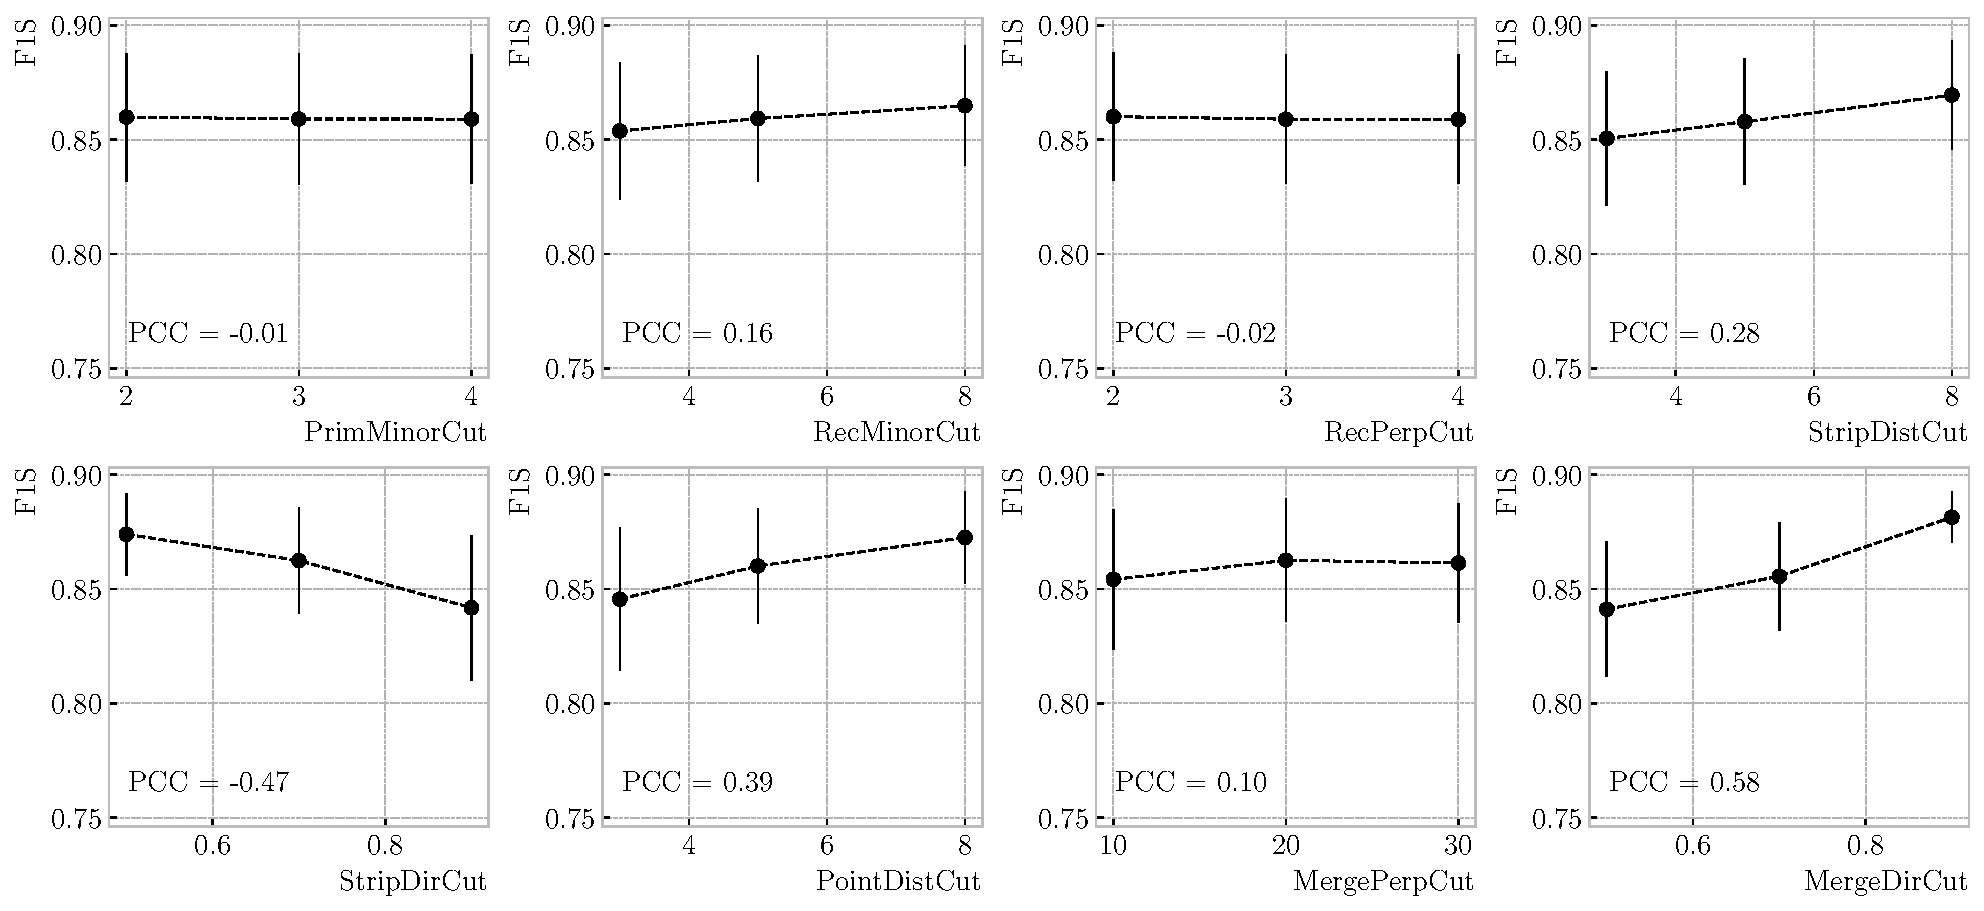
\includegraphics[width=.99\linewidth]{Images/GArSoft_Reco/cluster/coolcluster_optimisation_F1S.pdf}
	\caption{Mean values of the $F_{1}$-score marginal distributions for the different free parameters of the new clustering algorithm, with the error bars representing one standard deviation around the mean. The $F_{1}$-score values were computed for the 6561 possible parameter configurations using 1000 $\nu_{\mu}$ CC interaction events.}
	\label{fig:clustering_optimisation}
\end{figure}

\begin{table}[h!]
	\centering
	\caption{Summary of parameters and sampled values used in the optimisation of the clustering algorithm.}
	\begin{tabular}{l|l|l|p{7cm}}
		Name         & Units  & Sampled values & Description                                                                  \\ \hline
		PrimMinorCut & strips & 2, 3, 4        & Distance along strip length in NN clustering                                 \\
		RecMinorCut  & strips & 3, 5, 8        & Distance between propagated point and CM along strip length in re-clustering \\
		RecPerpCut   & strips & 2, 3, 4        & Closest hit pair distance in re-clustering                                   \\
		StripDistCut & strips & 3, 5, 8        & Distance between CMs in strip cluster merging                                \\
		StripDirCut  & cos    & 0.5, 0.7, 0.9  & Main axes direction cut in strip cluster merging                             \\
		PointDistCut & tiles  & 3, 5, 8        & Distance between propagated point and CM in strip-tile matching              \\
		MergePerpCut & cm     & 10, 20, 30     & Closest hit pair distance in module merging                                  \\
		MergeDirCut  & cos    & 0.5, 0.7, 0.9  & Main axes direction cut in module merging                                   
	\end{tabular}
	\label{tab:clustering_optimisation}
\end{table}

This algorithm has a total number of eight free parameters that need to be optimised. I used a sample of 1000 $\nu_{\mu}$ CC interactions in order to obtain the optimal configuration of clustering parameters. This sample was generated up to the default ECal hit clustering level, so then I could run the new clustering algorithm each time with a different configuration of parameters. As the number of parameters is relatively large, I only performed a coarse-grained scan of the parameter space. Sampling each of the eight parameters at three different points each I obtain 6561 different configurations. These parameters, together with the used values, are summarised in Tab. \ref{tab:clustering_optimisation}.

In order to measure the performance of the clustering, I use a binary classification approach. For each formed cluster, I identify the Geant4 Track ID of the matching MC particle and the energy fraction of each hit. Then, I assign to each cluster the Track ID with the highest total energy fraction. For each of the different Track IDs associated to the clusters, I select the cluster with the highest energy (only from the hits with the same Track ID). I identify such a cluster as the main cluster for that Track ID. I count as true positives (TPs) the hits with the correct Track ID in each main cluster. False positives (FPs) are the hits with the incorrect Track ID for the cluster they are in, not only main clusters. The false negatives (FNs) are the hits with the correct Track ID in clusters other than the main.

Fig. \ref{fig:clustering_optimisation} shows the computed $F_{1}$-score values for the different cuts. In each case, the central value represents the mean of the $F_{1}$-score distribution for the specified value of the corresponding variable and the vertical error bar represents one standard deviation around the mean. Also shown are the Pearson correlation coefficients of these central values. We can see that five of the variables have a sizeable effect on the $F_{1}$-score, with an absolute difference between the last and first values as big as $4\%$.

The working configuration is obtained as follows. I first select all configurations with purity $\geq90\%$. Among those, I choose the combinations that yield the maximum $F_{1}$-score. If more than one configuration remains I select the one with the highest sensitivity. Doing so, I end up with a parameter configuration with an efficiency of $88\%$ and a $90\%$ purity. Compared with the default algorithm, which gives an efficiency of $76\%$ and a purity of $91\%$ for the same sample, I have managed to improve the efficiency by a factor of $1.16$.

\begin{figure}[t]
	\begin{subfigure}{0.5\textwidth}
		\centering
		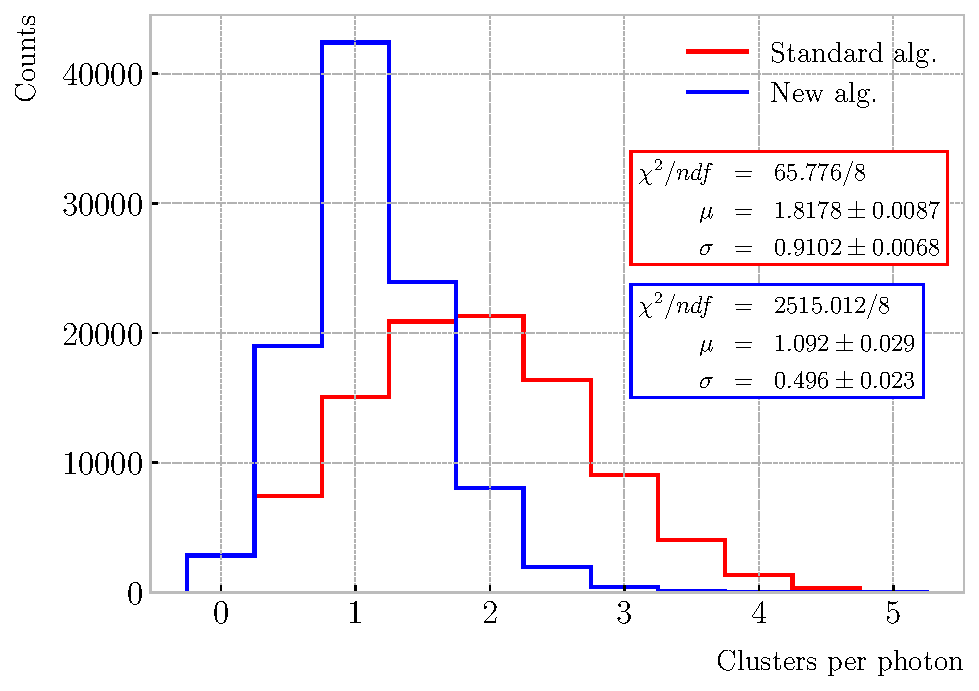
\includegraphics[width=.99\linewidth]{Images/GArSoft_Reco/cluster/coolcluster_clusters_per_photon.pdf}
	\end{subfigure}
	\begin{subfigure}{0.5\textwidth}
		\centering
		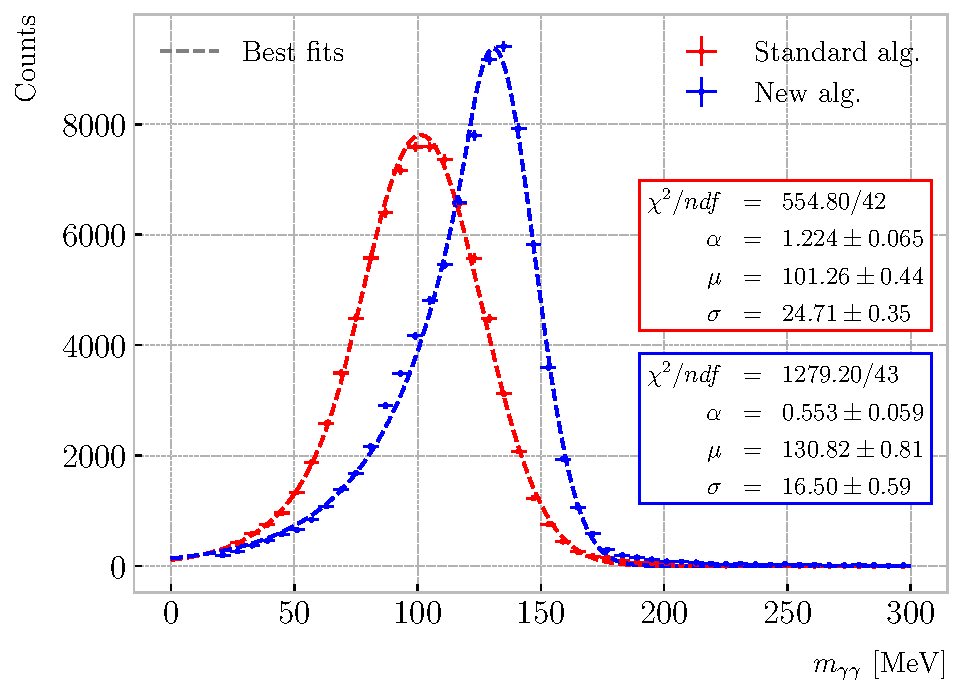
\includegraphics[width=.99\linewidth]{Images/GArSoft_Reco/cluster/coolcluster_invariant_mass_vertex.pdf}
	\end{subfigure}
	\caption{Left panel: distributions of the number of ECal clusters per photon from $\pi^{0}$ decays for the standard (red) and new (blue) clustering algorithms. Right panel: reconstructed invariant mass distributions for photon pairs from single $\pi^{0}$ events using the standard (red) and new (blue) ECal clustering algorithms.}
	\label{fig:clustering_pizero}
\end{figure}

\subsection{Neutral pion reconstruction}

One of the potential applications of the new ECal hit clustering is the reconstruction of neutral particles, in particular pions. Neutral pions decay promptly after being produced, through the $\pi^{0} \rightarrow \gamma\gamma$ channel $(98.823 \pm 0.034)\%$ of the time. The photon pair does not leave any traces in the HPgTPC (unless one or both of them converts into an electron-positron pair), but each of them will produced an electromagnetic shower in the ECal.

To test the potential impact of the new algorithm in $\pi^{0}$ reconstruction, I generated a MC sample of single, isotropic neutral pions inside the HPgTPC. All pions were generated with a momentum $p = 500 \ \mathrm{MeV}$ and their initial positions were uniformly sampled inside a $2 \times 2 \times 2 \ \mathrm{m}$ box aligned with the centre of the TPC. I ran both the default and the new clustering algorithms, using for the latter the optimised configuration discussed above.

The first thing to notice is that the number of clusters produced per photon has decreased. Fig. \ref{fig:clustering_pizero} (left panel) shows these distributions for the default (red) and new (blue) algorithms. Using a simple Gaussian fit, we see that the mean number of ECal clusters per photon went from $1.82 \pm 0.01$ to $1.09 \pm 0.03$. This effectively means that with the new algorithm the ECal activity of one true particle is typically reconstructed as a single object. From the reconstruction point of view this can be an advantage. As now most of the photon energy ends up in a single ECal cluster, I can simply use cluster pairs to identify the $\pi^{0}$ decay.

In general, one calculates the invariant mass of the photon pair as:
\begin{equation}
	m_{\gamma\gamma} = \sqrt{2E_{1}E_{2}(1-\mathrm{cos} \ \theta)},
\end{equation}
where $E_{i}$ are the energies of the photons and $\theta$ the opening angle between them. In this case I can use the energies deposited in the ECal and their incident directions. This quantity is computed for all possible pairs of clusters, using their position together with the true decay point. In a more realistic scenario, e.g. $\nu_{\mu}$ CC interaction, one could use the position of the reconstructed primary vertex instead. I also tried to use the principal direction of the clusters, but that approach gave considerably worse results. For each event I only keep the pair with an invariant mass closer to the true $\pi^{0}$ mass value.

Fig. \ref{fig:clustering_pizero} (right panel) shows the invariant mass distributions for the photon pairs we get using the default (red) and the new (blue) ECal clustering algorithms. For the fit I used a modified version of the Crystal Ball function \cite{Gaiser1982}, obtained by taking the limit where the parameter controlling the power-law tail goes to infinity:
\begin{equation}
	f(x; N, \mu, \sigma, \alpha) = N \cdot
	\left\{
	\begin{array}{ll}
		\mathrm{e}^{\frac{\alpha(2x-2\mu+\alpha\sigma)}{2\sigma}};& x \leq \mu - \alpha\sigma,\\
		\mathrm{e}^{-\frac{(x-\mu)^{2}}{2\sigma^{2}}};& x > \mu - \alpha\sigma.
	\end{array}
	\right.
\end{equation}
Comparing the fitted mean and standard deviation values for the Gaussian cores, we see that the distribution for the new algorithm is a $67\%$ narrower and also peaks much closer to the true $m_{\pi^{0}}$ value, going from $101.3 \pm 0.4 \ \mathrm{MeV}$ to $130.8 \pm 0.6 \ \mathrm{MeV}$.

\section{TPC track - ECal cluster matching}

One of the main players in the particle identification, in particular for muon and pion separation, is the way we associate clusters in the ECal to reconstructed tracks in the TPC. Missing some associations or making wrong ones can bias the ECal quantities that we can use for classifying particles. The current algorithm in GArSoft provides precise associations, i.e. most of the associations that it produces are correct, but it appears to miss an important number of associations (at least when using the default configuration).

The current TPC track-ECal cluster association algorithm is divided in four parts. It first checks whether the track end point fulfils certain conditions to be extrapolated. There are two cut values in this step, one for the drift direction and other radial.

If the point can be extrapolated, the code computes the coordinates of the centre of curvature using the Kalman fit estimates at the track end $(y, \ z, \ 1/R, \ \phi, \ \mathrm{tan}\lambda)$. It then compares the distance between this and the cluster in the $(z,y)$ plane with $R$. This introduces another cut in the perpendicular direction.

The next step is different for clusters is in the barrel or in one of the end caps. If it is a barrel cluster the algorithm extrapolates the track up to the radial distance of the cluster. There are three possible outcomes, the extrapolated helix can cut the cylinder of radius $r_{clus}$ two, one or zero times. I get the cut point that is closer to the cluster and check that it is either in the barrel or the end caps. Computing the difference between the $x$ coordinates of the cluster and the extrapolated point, the module checks that this is not greater than a certain cut. If the cluster is in an end cap, I propagate the track up to the $x$ position of the cluster. Then, the algorithm computes the angle in the $(z,y)$ plane between the centre of curvature and the cluster, $\alpha$, and the centre of curvature and the propagated point, $\alpha'$. A cut is applied to the quantity $(\alpha-\alpha')R$.

If the cluster contains more than a certain number $N$ of hits, I apply an extra cut to the dot product of the direction of the track at the propagated $x$ value and the cluster direction.

The code makes sure to only associate one end of the track (if any) to a cluster. However, it can associate more than one track to the same cluster. This makes sense, as different particles can contribute to the same cluster in the ECal, but it makes it difficult to quantify the relative contributions of the tracks to a certain cluster.

As a way of comparing the performance of this algorithm, a new, simpler association module was written. The goal was to have a simple and robust algorithm, which depends on as few parameters as possible and that can produce a one-to-one matching between tracks and ECal clusters.

\begin{figure}[t]
	\begin{subfigure}{0.5\textwidth}
		\centering
		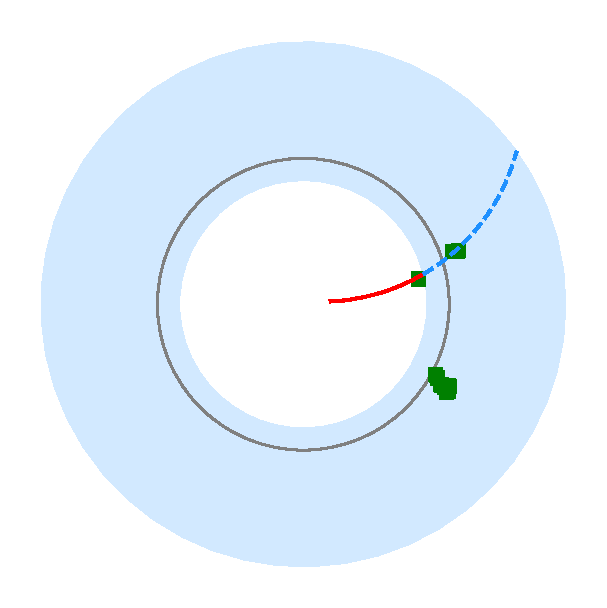
\includegraphics[width=.85\linewidth]{Images/GArSoft_Reco/associations/helix_propagation_example.pdf}
	\end{subfigure}
	\begin{subfigure}{0.5\textwidth}
		\centering
		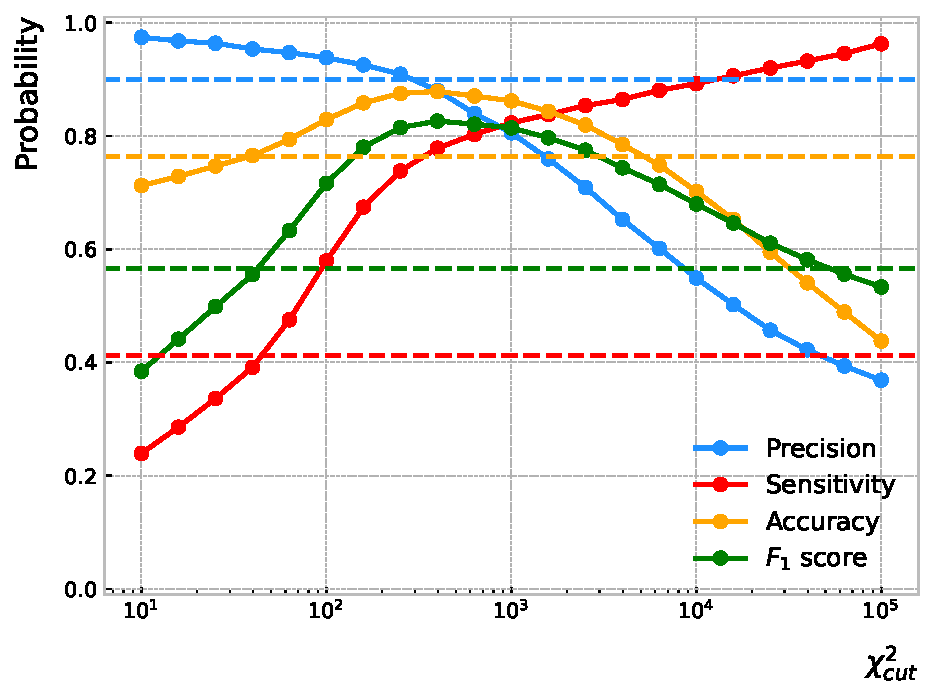
\includegraphics[width=.99\linewidth]{Images/GArSoft_Reco/associations/helix_propagation_metrics_2.pdf}
	\end{subfigure}
	\caption{Left panel: example reconstructed track (red line) propagated up to an angle $\phi_{max} = \pi/2$ (dashed blue line). Also shown are the ECal clusters in the event (green squares). Right panel: performance metrics.}
	\label{fig:associations}
\end{figure}

For each reconstructed track, the new algorithms applies the same procedure to the forward and the backward fits irrespective of their end point positions. It first gets the Kalman fit parameters at the corresponding end point together with the $X$ position, $x_{0}$, $(y_{0}, \ z_{0}, \ 1/R, \ \phi_{0}, \ \mathrm{tan}\lambda)$.

For each ECal cluster, I compute the radial distance to the centre of the TPC and find the $\phi$ value in the range $[\phi_{0}, \ \phi_{0}+\mathrm{sign}(R)\phi_{max})$ that makes the propagated helix intersect with the circle defined with such radius. The $(x,y,z)$ position of the helix for the $\phi$ value found (if any) is then computed. In case there are two intersections, I keep the one that minimises the distance between $(y, z)$ and $(y_{c}, z_{c})$.

Fig. \ref{fig:associations} (left panel) shows an example track (red line) being propagated up to $\phi_{0}+\mathrm{sign}(R)\pi/2$ (dashed blue line). The image also shows the ECal clusters present in the event (green squares). For each of them, the algorithm will try to find the intersections of the propagated helix and the circles defined with their corresponding radii.

I then calculate $\chi^{2}$ value based on the Euclidean distance between the propagated point and the cluster:
\begin{equation}
	\chi^{2}/ndf = \frac{\sum_{n=0}^{2}\left(x^{(n)}-x^{(n)}_{c}\right)^{2}}{3}.
\end{equation}
If there was no intersection I store a $-1$ instead. In the end, for each reconstructed track in the event one ends up with two collections of $\chi^{2}$ values, one for each ECal cluster and fit directions.

The current code only supports having ECal clusters associated to one end of each track. We have two options to decide what track end to keep. The first one tries to cheat the selection, looking at the distance between the two track ends and the true start position of the associated MC particle. The second one keeps the track end with more $\chi^{2}$ entries below the cut.

This feature of only considering one track end limits the algorithm, making it not suitable for reconstructing events with particles originating outside the TPC. However, as for the moment the main concern of the group is the study of neutrino interactions off the gaseous argon, this is an acceptable assumption.

In order to associate a cluster to a track, I take all clusters with a $\chi^{2}$ value in the range $[0, \chi^{2}_{cut})$. If a cluster has been assigned to more than one track we leave it with the one with the lowest $\chi^{2}$.

This default behaviour of the algorithm can be modified to associate more than one track to each cluster. Not only that, but the $\chi^{2}$ values can be used to assign relative weights to the different contributions.

To evaluate the performance of the association method, I use a binary classification approach. In this case, I check the leading MC Track IDs associated to the reconstructed tracks and ECal clusters. I count an association as true positive (TP) if both Track IDs coincide. An association is considered false positive (FP) when the Track IDs are different. If a cluster has not been associated to any track but it shares the Track ID with a reconstructed track it is counted as a false negative (FN).

Fig. \ref{fig:associations} (right panel) shows the precision (blue line), sensitivity (red line), accuracy (orange line) and $F_{1}$-score (green line) for different values of $\chi^{2}_{cut}$. For comparison, the same metrics computed for the default algorithm with the current configuration are also shown (dashed lines). Notice that we can achieve similar values of the precision with this new code while having a considerably higher sensitivity.

\begin{figure}[t]
	\centering
	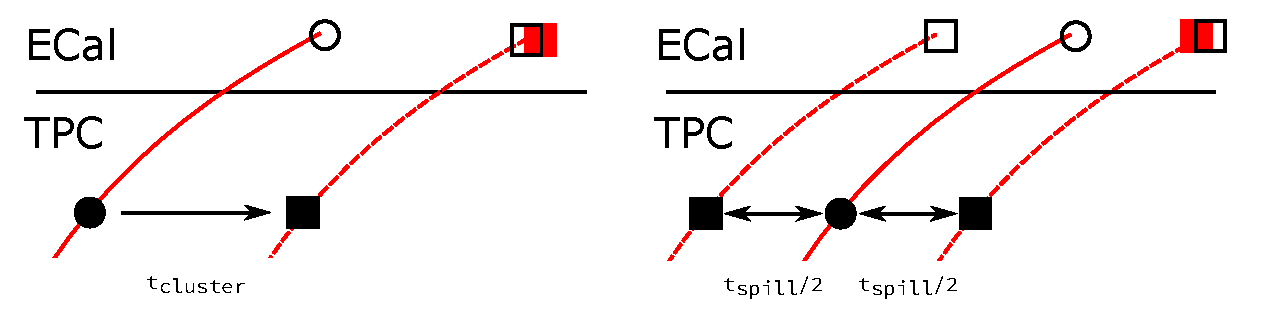
\includegraphics[width=.99\linewidth]{Images/GArSoft_Reco/associations/drift_correction.pdf}
	\caption{Schematics of possible options to deal with track-ECal associations in non-zero $t_{0}$ neutrino interaction events. The first option (left panel) tries to correct for the drift direction uncertainty in a cluster-by-cluster basis using the cluster time, $t_{cluster}$. The second option (right panel) is based on a track-by-track approach, propagating two additional helices for each track corrected by factors of $\pm t_{spill}/2$.}
	\label{fig:associations_drift}
\end{figure}

One of the possible weak points of this approach is that it relies on the position along the drift direction to make the decisions. Within the current ND-GAr design implemented in GArSoft, the timing information is provided by the ECal. That effectively means that prior to make the track-ECal associations the reconstructed $X$ positions of the track trajectories differ from the simulated ones by an amount:
\begin{equation}
	x_{reco}^{(n)} - x_{sim}^{(n)} = v_{drift} \ t_{0},
\end{equation}
where $v_{drift}$ is the mean drift velocity in our medium and the initial time is in the range $t_{0}\in[0, t_{spill})$ where $t_{spill}$ is the spill length. For a $10 \ \mu\mathrm{s}$ spill this translates into a maximum $30 \ \mathrm{cm}$ uncertainty on the drift direction position.

The current default in GArSoft sets $t_{0} = 0$, but the functionality to randomly sample this within the spill time is in place. Therefore, we need to understand what is the impact of a non-zero $t_{0}$ on the associations algorithm and foresee possible ways of minimising a loss in performance.

Fig. \ref{fig:associations_drift} represents two different options to tackle the associations problem when having events with a non-zero initial time $t_{0}$. The circles represent the original points, whereas the squares indicate the corrected positions. The end points of the track and the propagated points up to the cluster radius are indicated using filled and unfilled markers respectively. The red square represents the position of the cluster.

In the first option (left panel) I try to correct for the drift coordinate position using the time associated to the cluster. Assuming that the drift time is much larger than the propagation time, $t_{cluster}$ could be used as a good estimation of the $t_{0}$. An alternative can be using the earliest time associated to a hit in said cluster. Doing this for each cluster before computing the $\chi^{2}$ value could be used as an alternative to knowing the specific value of the $t_{0}$, as when the association is correct this will provide the right correction but its impact is small enough to not change the position significantly in the case the cluster does not correspond to a given track.

The second method depicted in Fig. \ref{fig:associations_drift} (right panel) tries to propagate three different helices for each reconstructed track and fit direction. One is the original, uncorrected helix and the other two are obtained by adding factors of $\pm t_{spill}/2$ when computing the drift coordinate position. In this case one would compute a set of $\chi^{2}$ values for each helix, keeping in the end the collection that manages to keep more values below $\chi^{2}_{cut}$. An alternative approach could be using a family of helices instead, using uniformly sampled time correction values in the $\pm t_{spill}/2$ range.

Both options could offer a solution to the $t_{0}$ problem, and still need to be explored.

All the topics discussed in this Chapter represent the main changes I made to the reconstruction in GArSoft. They were motivated by the need of a PID and in particular the reconstruction of the pion multiplicity. I introduced each of them pointing out how they relate to the PID and showed that the proposed solution manages to tackle the specific problem. The only point that is missing is to demonstrate the impact these changes have on the PID and the pion multiplicity. That is my main priority at the moment, as once that is understood I will be able to generate the new samples to be used in the LBL analysis.